\documentclass{article}
\usepackage[margin=0.8in]{geometry} % Set margins to 0.8 inch
\usepackage{graphicx} % Required for inserting images
\usepackage{hyperref}
\usepackage{tabularx}
\usepackage{amsmath}
\usepackage{amssymb}
\usepackage{float}
\usepackage{listings}
\usepackage{xcolor}
\usepackage[backend=biber,style=ieee,]{biblatex}

\lstset{
  basicstyle=\ttfamily\footnotesize,
  breaklines=true,
  breakatwhitespace=true,
  frame=single,
  numbers=left,
  numberstyle=\tiny,
  keywordstyle=\color{blue},
  commentstyle=\color{gray},
  stringstyle=\color{red},
  tabsize=4,
  captionpos=b,
  mathescape=true,
  literate={_}{\_}1  % <-- add this line
}

\addbibresource{ref.bib}


\setlength{\parindent}{0pt}

\title{
    \Huge \textbf{Self-Balancing Robot}

    \vspace{100px}

    \large Course: ELEC 391 201 2024W2 \\[1em]
    \large Authors: Team B-17 (Tomaz Zlindra, Muntakim Rahman, Xianyao Li) \\[1em]
    \large Instructors: Dr.\ Joseph Yan and Dr.\ Cristian Grecu \\[1em]
    \large Submission Date: April 13th, 2025 \\
}

\date{} % Remove default date

\begin{document}

\pagenumbering{gobble} % Suppress page numbering for the title page
\maketitle

\newpage % Start numbering after title page
\pagenumbering{arabic} % Restart numbering at 1

\tableofcontents % Generate Table of Contents

\newpage % Start main content

\section{Introduction}

• Description of the engineering problem or challenge
• Background context and any relevant history

\section{Requirements, Specifications and Constraints}

\subsection{Functional Requirements}

Table~\ref{tab:functional_requirements} lists the functional requirements of the self-balancing robot. These are prioritized by category,
either a core or additional feature. The core functionality of the robot relates to its ability to autonomously balance itself and be driven
by a human user via Bluetooth. The additional features were designed to enhance the robot's capabilities, in detecting environmental factors and
providing useful information to the user.

\begin{table}[H]
    \centering
    \renewcommand{\arraystretch}{1.3} % Increase row height for readability
    \begin{tabularx}{\textwidth}{|c|X|c|}
        \hline
        \textbf{ID} & \textbf{Requirement Description} & \textbf{Priority} \\
        \hline
        FR1 & The robot must balance on a flat surface by controlling the DC motors. & Core \\
        \hline
        FR2 & The robot must maintain balance while driven externally on a flat surface. & Core \\
        \hline
        FR3 & The robot must maintain balance while turning at a reasonable speed. & Core \\
        \hline
        FR4 & The robot must move forward and backward under external control. & Core \\
        \hline
        FR5 & The robot must be controlled via Bluetooth with four directional commands. & Core \\
        \hline
        FR6 & The robot must be able to recover when disturbed & Core \\
        \hline
        FR7 & The robot is powered solely by a pack of 8 $\times$ 1.2V rechargeable batteries. & Core \\
        \hline
        FR8 & The distance sensor must detect obstacles and stop when it gets too close to an object & Additional Feature \\
        \hline
        FR9 & The color sensor must be able to detect at least one color & Additional Feature \\
        \hline
        FR10 & The RFID module must authenticate an RFID tag and prevent unauthorized operation. & Additional Feature \\
        \hline
        FR11 & The Raspberry Pi Zero must process and transmit a camera feed through Pi Connect & Additional Feature \\
        \hline
        FR12 & The AWS Bucket should store all the saved images and videos from the camera & Additional Feature \\
        \hline
    \end{tabularx}
    \caption{Functional Requirements of the Self-Balancing Robot}
    \label{tab:functional_requirements}
\end{table}

\subsection{Performance Requirements}
Table \ref{tab:performance_requirements} outlines the performance requirements for the self-balancing robot, providing specific quantitative targets to assess the system's effectiveness. These requirements closely align with the functional requirements, but with the addition of measurable criteria—such as recovery angle, speed and transmission speed. By translating functional goals into performance metrics, we ensured that the robot’s behavior could be consistently validated against clearly defined benchmarks. This approach helped guide both the design process and iterative improvements throughout development.

\begin{table}[H]
    \centering
    \renewcommand{\arraystretch}{1.3} % Increase row height for readability
    \begin{tabularx}{\textwidth}{|c|X|c|}
        \hline
        \textbf{ID} & \textbf{Requirement Description} & \textbf{Priority} \\
        \hline
        PR1 & The robot must respond to a 15 degree disturbance and re-balance & Core \\
        \hline
        PR2 & The robot must maintain balance with a positional drift of less than 15 cm over 10 seconds on a flat surface. & Core \\
        \hline
        PR3 & The Bluetooth latency for control commands must be less than 100 ms. & Core \\
        \hline
        PR4 & The robot must be able to maintain a Bluetooth connection within a range of at least 5 meters. & Core \\
        \hline
        PR5 & The robot must be to move forward, backward, left (45$^\circ$) and right (45$^\circ$) within 5 seconds & Core \\
        \hline
        PR6 & The obstacle detection system must stop the robot within 1 cm of an obstacle detected between 2–30 cm. & Additional Feature \\
        \hline
        PR7 & The color sensor must identify red and respond accordingly within 100ms & Additional Feature \\
        \hline
        PR8 & The RFID reader must successfully detect and authenticate tags within 1 second. & Additional Feature \\
        \hline
        PR9 & The Raspberry Pi Zero must transmit a camera feed at no less than 1 FPS. & Additional Feature \\
        \hline
    \end{tabularx}
    \caption{Performance Requirements of the Self-Balancing Robot}
    \label{tab:performance_requirements}
\end{table}

\subsection{Constraints}

\subsubsection{Financial}
This project operated under a strict financial constraint, with a maximum budget of \$65 allocated specifically for additional features (excluding taxes and shipping). To maximize the number of features within this limit, we opted to purchase components from alternative vendors when they offered more competitive prices than DigiKey. We determined that the most effective use of our budget was to prioritize implementing multiple smaller features, rather than allocating the entire amount toward a single major feature.

\

For a detailed breakdown of the expenses, refer to the \href{https://docs.google.com/spreadsheets/d/1k2FMDTlyxH50N65zvA1Ss5obWOlDuc3JaWVVDWrQ88E/edit?usp=sharing}{Google Sheet with all financial details} An image can also be found in the Appendix in Figure \ref{fig:financials}.

\subsubsection{Temporal}

Although the final project deliverable was due on April 8th, 2025, we set several soft deadlines along the way to track our progress and prevent last-minute workload buildup. Some of the main deadlines are shown below.

\begin{description}
  \item[February 28th, 2025] Motor Control PWM for Arduino
  \item[March 6th, 2025] Completed BLE Integration with Python App
  \item[March 7th, 2025] Completed Distance Sensor and Color Sensor STM32 Firmware
  \item[March 13th, 2025] Completed PID k-value Calculations
  \item[March 14th, 2025] Completed RFID STM32 Firmware
  \item[March 20th, 2025] Completed Raspberry Pi App
  \item[March 21st, 2025] Completed Speaker Integration STM32 Firmware
  \item[March 28th, 2025] Completed Robot Balancing
\end{description}

Although most deadlines were met, a few, particularly the robot balancing milestone were not achieved on time. This delay was primarily due to some questionable firmware design decisions that introduced unforeseen challenges. Fortunately, these issues were resolved, and the system was successfully completed in the end.


\subsubsection{Materials}
For the custom construction of our self-balancing robot, we were limited to using thick plastic for laser cutting and standard 3D printing filament, as these materials were readily available and did not impact our budget. While other materials—such as aluminum, carbon fiber, or specialized fasteners—could have offered enhanced strength or reduced weight, they would have required additional spending from our \$65 budget. To stay within our constraints, we opted not to purchase any external materials and instead focused on optimizing our design using the provided components and available fabrication methods.

\subsubsection{Environmental}
The performance of a self-balancing robot can be significantly affected by environmental constraints such as battery levels, electromagnetic interference (EMI), temperature, and terrain conditions. Low battery voltage can reduce motor torque and sensor accuracy, leading to instability. EMI from nearby motors or power electronics can disrupt IMU readings and communication systems, making balance control less reliable. Temperature extremes can alter sensor calibration and battery efficiency, while uneven or slippery terrain can interfere with traction and cause the robot to lose balance. These factors must be carefully considered to ensure reliable operation in real-world environments.

\section{Conceptual Design}

\subsection{High-level Functional Diagram}

\begin{figure}[H]
    \centering
    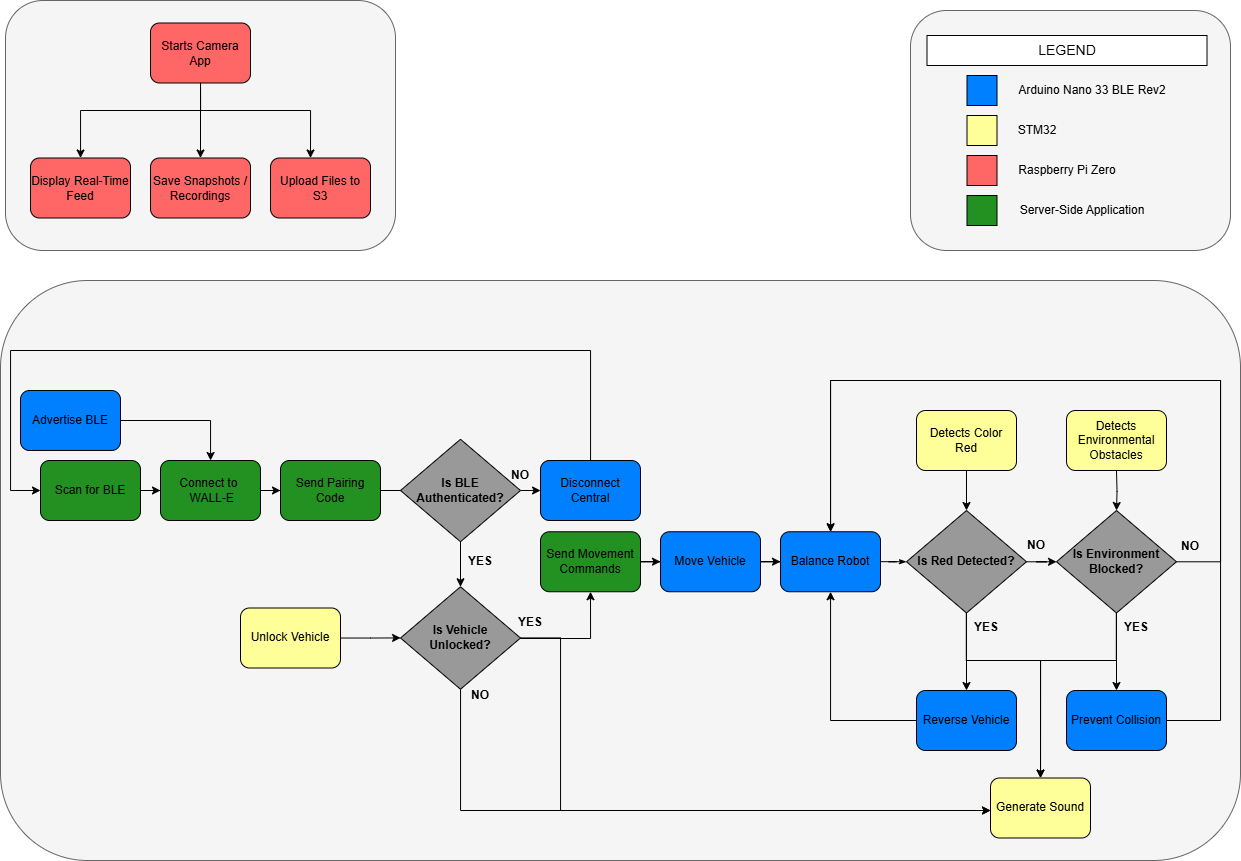
\includegraphics[width=1\textwidth]{Figures/Functional_Diagram.png}
    \caption{High-level Functional Diagram}
    \label{fig:functional_diagram}
\end{figure}

\begin{minipage}{\linewidth}
    The functional diagram in Figure~(\ref{fig:functional_diagram}) highlights our system-design for enforcing secure access of the robot with
    \textbf{RFID} and \textbf{Bluetooth Low Energy (BLE)}. We prevent users from balancing or moving the robot without the required authentication. Once successful,
    the firmware was programmed to prioritize safe operation of the robot, while accounting for environmental factors such as distance and color detection. \\
\end{minipage}

\subsection{Architecture Diagram}

\begin{figure}[H]
    \centering
    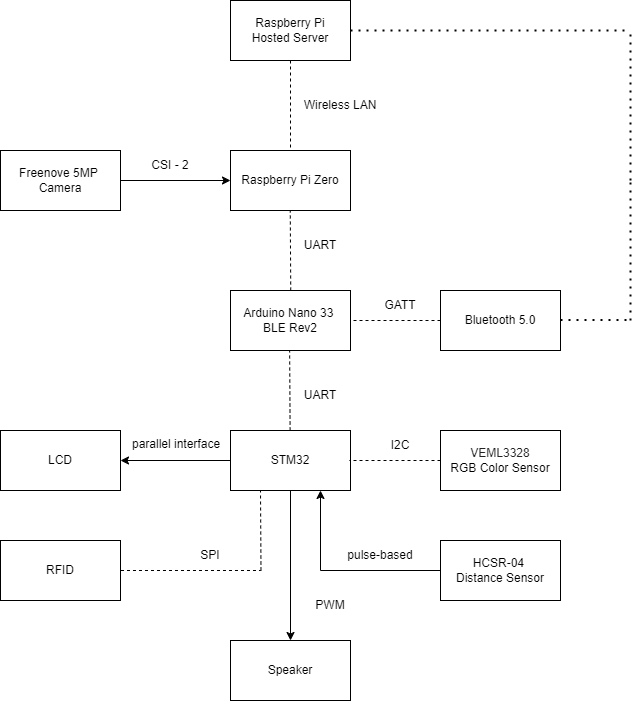
\includegraphics[width=0.7\textwidth]{Figures/Architecture_Diagram.png}
    \caption{Architecture Diagram}
    \label{fig:architecture_diagram}
\end{figure}

\begin{minipage}{\linewidth}
    The architecture diagram in Figure~(\ref{fig:architecture_diagram}) describes the interfaces between robot peripherals and the three boards
    used in the project: \\
\end{minipage}

\begin{itemize}
    \item \textbf{Arduino Nano 33 BLE Sense Rev2} was responsible for driving the motors and maintaining balance.
    \item \textbf{STM32L051K8T6} was responsible for environmental detection and physical authentication.
    \item \textbf{Raspberry Pi Zero W} was responsible for displaying and processing camera input for the user.
\end{itemize}

\textit{Note that we wirelessly accessed the \textbf{Raspberry Pi} and \textbf{Arduino} from a development machine.}

\section{Subsystem Design}

\subsection{Structural Design}

\subsubsection{Design Decisions}
Since the transfer function of the robot was derived under the assumption that
the center of mass of the pendulum is perfectly centered, the structural design
follows the principle of evenly distributing mass to ensure that the center of
mass is as close as possible to the rotor axis.

\


Another design decision we made was to mount the third layer as high as
possible. This choice addresses the fact that the plant is a nonlinear and
inherently unstable system, which can only be effectively controlled within a
region where it can be approximated as linear. To evaluate the impact of the
third layer's height on system behavior, we simulated the plant's step response
at different mounting heights:

\begin{figure}[H]
    \centerline{\fbox{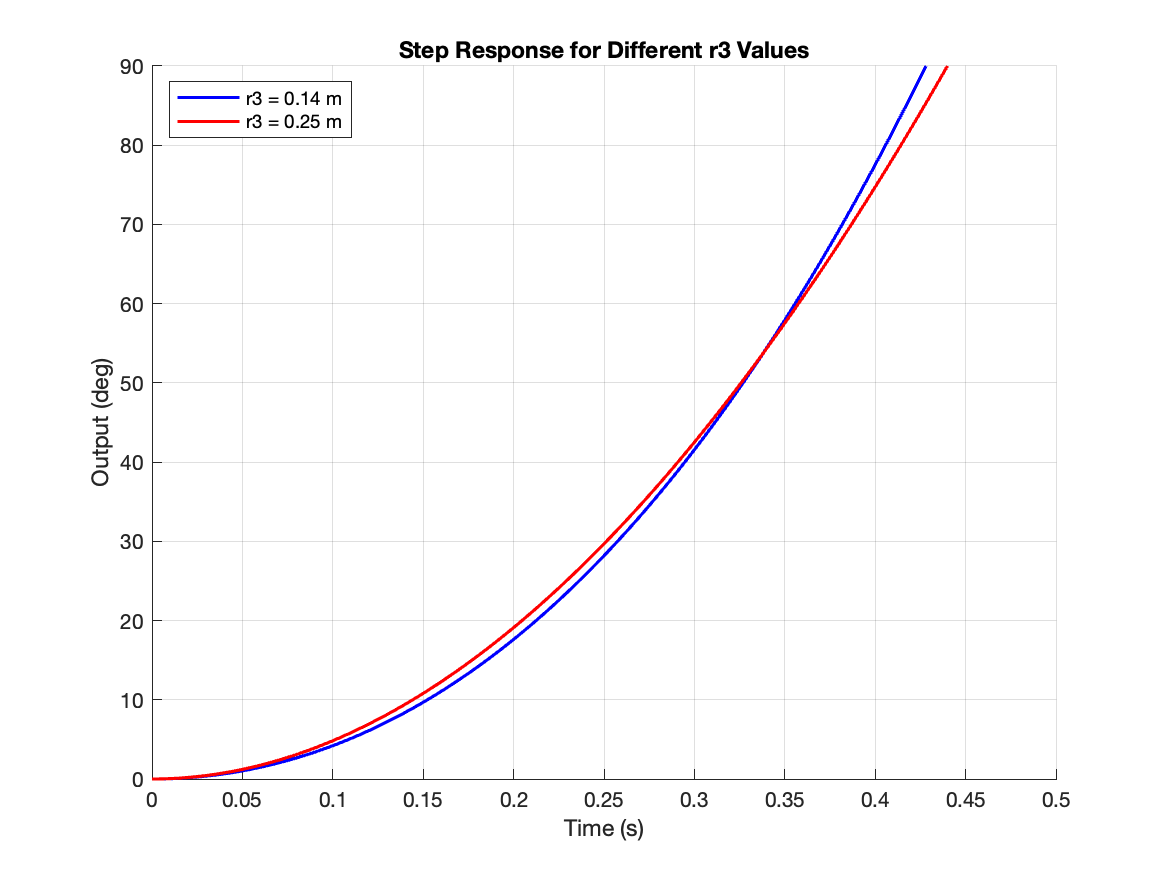
\includegraphics[width=0.65\linewidth]{Figures/r3step.png}}}
    \caption{Step Response of the Plant with Different Height of the Third Layer}
\end{figure}

As shown in the figure, increasing the height of the third layer results in a
step response that more closely resembles that of a linear system, making it
easier to control.

\begin{figure}[H]
    \centerline{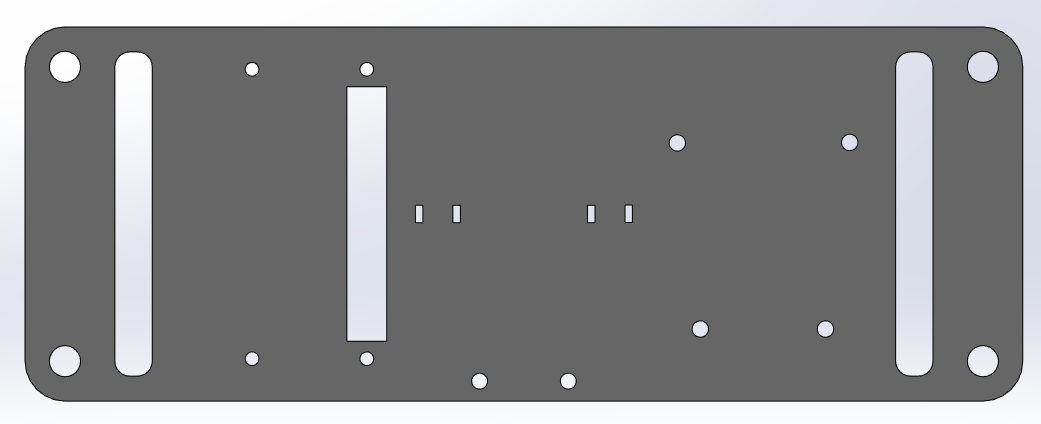
\includegraphics[width=\linewidth]{Figures/3rdlayer.png}}
    \caption{Design of the Third Layer}
\end{figure}

\subsubsection{Third Layer Design}
On the third layer, we need to mount the Raspberry Pi, color sensor, RFID
reader, and camera. The four mounting holes on the left side are for securing
the Raspberry Pi, while the four holes on the right are for the RFID reader.
These holes are positioned to ensure that both components are centered relative
to the third layer once mounted.

At the bottom, two mounting holes are used to attach the L-stand for the color
sensor. Since we only have one color sensor, its placement causes a deviation in
the center of mass. To compensate for this imbalance, the camera is zip-tied at
the center, allowing its position to be adjusted to help realign the center of
mass. Although not shown in the figure, two distance sensors are also mounted on
the second layer symmetrically.

\subsubsection{L-stand Design}
The design of the L-stand is shown below:
\begin{figure}[H]
    \centerline{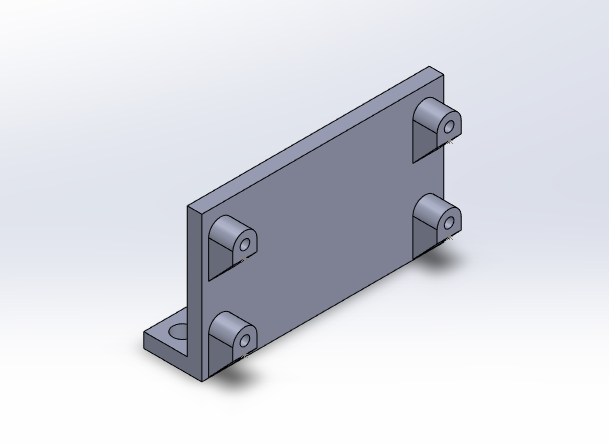
\includegraphics[width=0.5\linewidth]{Figures/standDis.png}}
    \caption{Design of the L-stand for Mounting the Distance Sensor}
\end{figure}

The L-stand includes four columns to provide clearance for the distance sensor,
as there are components located on the back of the PCB. Ribs are added beneath
each column to address potential issues during 3D printing. Since overhangs can
lead to poor print quality or failed prints, the ribs provide structural support
under the columns, eliminating overhangs and making the printing process more
reliable and efficient.

\

The L-stand for the color sensor follows the same design principles with
different dimension, thus is not shown here.

\subsection{PID Modeling and Simulation}
\subsubsection{Measuring Robot Parameters}

With the corrected transfer function, we need to find the values of the
parameters in order to get the transfer function. \\

We start with the motor constants. For $K_t$, from the datasheet we know
that the stall current is 5.5 A and the torque at 12 V is 85 kg$\cdot$mm, or
0.83N$\cdot$m, we can then get the value of $K_t$ by dividing the torque by the
stall current, which is 0.1516. \\

For $K_e$, from the datasheet we know that the free run speed of the rotor
without the gearbox is 1047.19 rad/s, we can then get the value of $K_e$ by
dividing the load voltage 12 V by the free run speed of the rotor, which is
0.01146. \\

To obtain the moment of inertia of the pendulum $J_p$, we need to simplify the
plant model. The robot consists of four rods and three layers. Assuming the
center of mass is perfectly centered, the four rods can be approximated as a
single equivalent rod located at the center of the three layers. Similarly, the
three layers can be modeled as three point masses, which are further simplified
into a single point mass located at their collective center of mass. The
resulting simplified model consists of a single rod rotating about one end and a
point mass positioned at the center of mass of the three layers. \\
\begin{figure}[H]
    \centerline{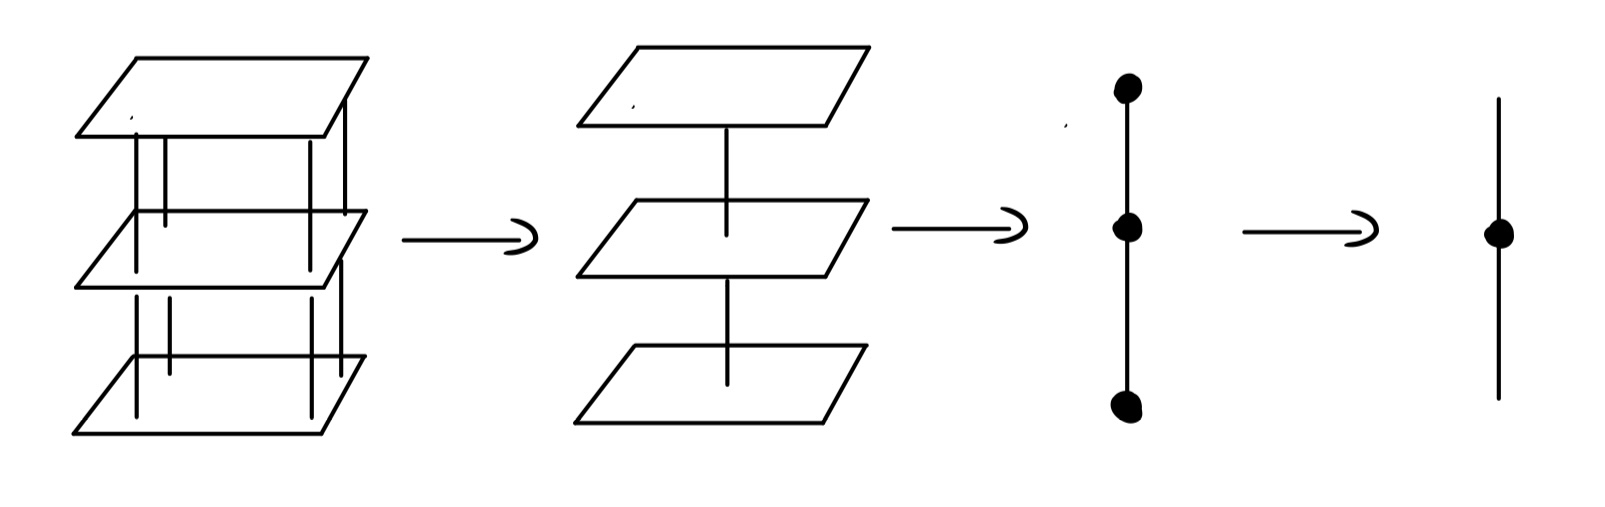
\includegraphics[width=\linewidth]{Figures/plantModelSimplification.png}}
    \caption{Simplification of the Plant Model}
\end{figure}

All of the other parameters can either be measured directly, or are negligible
and have minimal impact on the overall transfer function. \\

\subsubsection{Transfer Function}

Considering the difficulty of deriving the transfer function from first
principles, and given the abundance of studies on the same topic, we chose to
reference a published paper for guidance \cite{suspaper}. However, upon
reviewing the paper, we identified errors in part of the derivation: \\

Assuming the correctness of
\begin{align}
K_t \frac{V_s - K_e \dot{\theta}_m}{R_a} &= J_m \ddot{\theta}_m + \tau_w + b \dot{\theta}_m \\
\tau_w &= J_w \ddot{\theta}_w - F_{pH} r_w + m_w \ddot{\theta}_w r_w^2 \\
F_{pH} &= m_p (r_w \ddot{\theta}_w + l_g \ddot{\theta}_p) \\
F_{pH} l_g &= J_p \ddot{\theta}_p \\
\theta_m &= \frac{\theta_w}{G_r}
\end{align}
Substitute (3) into (4) gives:
\begin{align*}
m_p (r_w \ddot{\theta}_w + l_g \ddot{\theta}_p) l_g &= J_p \ddot{\theta}_p \\
m_p l_g r_w \ddot{\theta}_w + m_p l_g^2 \ddot{\theta}_p &= J_p \ddot{\theta}_p \\
m_p l_g r_w \ddot{\theta}_w &= (J_p - m_p l_g^2) \ddot{\theta}_p \\
\ddot{\theta}_w &= \frac{J_p - m_p l_g^2}{m_p l_g r_w} \ddot{\theta}_p \\
\theta_w &= \frac{J_p - m_p l_g^2}{m_p l_g r_w} \theta_p
\end{align*}
So Eq. 4 in the paper is incorrect. The \(\tau_w\) in denominator should be \(r_w\). The signs are also wrong.
Substitute (3) into (2) gives:
\begin{align*}
\tau_w &= J_w \ddot{\theta}_w - m_p (r_w \ddot{\theta}_w + l_g \ddot{\theta}_p) r_w + m_w \ddot{\theta}_w r_w^2 \\
&= (J_w + (m_w - m_p) r_w^2) \ddot{\theta}_w - m_p l_g r_w \ddot{\theta}_p
\end{align*}
Substitute the above and (5) into (1) and expand the first fraction:
\[
\frac{K_t}{R_a} V_s - \frac{K_t}{R_a} \frac{K_e}{G_r} \dot{\theta}_w - \frac{b}{G_r} \dot{\theta}_w - (J_w + (m_w - m_p) r_w^2) \ddot{\theta}_w + m_p l_g r_w \ddot{\theta}_p = \frac{J_m}{G_r} \ddot{\theta}_w
\]
Move the angle terms to RHS and flip both sides:
\begin{align*}
\left( \frac{K_t}{R_a} \frac{K_e}{G_r} + \frac{b}{G_r} \right) \dot{\theta}_w + \left[ \frac{J_m}{G_r} + J_w + (m_w - m_p) r_w^2 \right] \ddot{\theta}_w - m_p l_g r_w \ddot{\theta}_p &= \frac{K_t}{R_a} V_s
\end{align*}
Substitute the expression of \(\theta_w\) in terms of \(\theta_p\):
\begin{align*}
(J_p - m_p l_g^2) \left( \frac{K_t}{R_a} \frac{K_e}{G_r} + \frac{b}{G_r} \right) \dot{\theta}_p + \left[ (J_p - m_p l_g^2) \left[ \frac{J_m}{G_r} + J_w + (m_w - m_p) r_w^2 \right] + (m_p l_g r_w)^2 \right] \ddot{\theta}_p \\= \frac{K_t}{R_a} (m_p l_g r_w) V_s
\end{align*}
Laplace transform:
\begin{multline*}
\theta_p(s) \left[ (J_p - m_p l_g^2) \left( \frac{K_t}{R_a} \frac{K_e}{G_r} + \frac{b}{G_r} \right) s + \left[ (J_p - m_p l_g^2) \left[ \frac{J_m}{G_r} + J_w + (m_w - m_p) r_w^2 \right] + (m_p l_g r_w)^2 \right] s^2 \right]
\\= \frac{K_t}{R_a} (m_p l_g r_w) V_s(s)
\end{multline*}
Hence the final transfer function:
\[
\frac{\theta_p}{V_s}(s) = \frac{\frac{K_t}{R_a} (m_p l_g r_w)}{\left[ (J_p - m_p l_g^2) \left[ \frac{J_m}{G_r} + J_w + (m_w - m_p) r_w^2 \right] + (m_p l_g r_w)^2 \right] s^2 + (J_p - m_p l_g^2) \left( \frac{K_t}{R_a} \frac{K_e}{G_r} + \frac{b}{G_r} \right) s}
\]
The definition of the parameters can be found in the paper. \\

Plug in the parameters we acquired, the resulting open loop transfer function is:
\[
\frac{\theta_p}{V_s}(s) = \frac{977.5}{s^2+0.3439s}
\]
Notice that the moment of inertia of the wheel and the rotor ($J_m \& J_r$) and
friction $b$ are approximated to zero, This is because their magnitudes are
negligible compared to other parameters in the system, thus they have
minimal impact on the overall transfer function.

\subsubsection{PID Parameter Calculation}

From the previously derived transfer function, we observe that the two open-loop
poles are located at 0 and -0.3439, indicating that the system is unstable. To
stabilize the system, a feedback control loop must be introduced to shift the
poles of the closed-loop transfer function to stable locations. To determine the
PID parameters, we can apply the pole placement method: \\

Assuming that we want the resulting poles to be placed at $P_A$ and $P_B$, the
denominator of the resulting transfer function is:
\[
(s-P_A)(s-P_B)
\]
This can be written explicitly as:
\[
s^2 - (P_A + P_B)s + P_AP_B
\]
With a PD controller, the characteristic equation is:
\[
s^2 + (K \cdot K_d - (P_1 + P_2))s + P_1P_2 + KK_p
\]
Where $P_1$ and $P_2$ are poles of the open loop transfer function, $K$ is the
DC gain of the transfer function, which is 977.5.

\

We can relate the above two equations and the following equations can be obtained:
\begin{align*}
    P_AP_B &=  P_1P_2 + KK_p\\
    -(P_A + P_B) &= KK_d - (P_1 + P_2)
\end{align*}
The resulting PD gains will make the close loop transfer function be critically
damped and stable.

\

To determine the desired pole locations, we first need to select an appropriate
time constant $N$. By measuring the runtime of the main control loop, we found
the worst-case execution frequency to be 25 Hz. According to the Nyquist
theorem, the sampling rate must be at least twice the highest frequency
component to accurately capture the system dynamics. Therefore, the maximum
allowable control bandwidth is 12.5 Hz, corresponding to a minimum time constant
of approximately 0.08. To ensure stability and responsiveness while staying
within this limit, we chose a time constant of 1/4 seconds, which places the
desired pole at $-8\pi$ and the resulting $K_p$ and $K_d$ are 0.6462 and 0.0511,
respectively.

\

The I term is added after to address the drifting issue we encountered during
the testing. The value of $K_i$ was found by trial and error, and the final
value of $K_i$ is 11.5.

\subsubsection{Simulink Simulation}

Simulink is used to validate the design of the PID controller. The model is
shown below:
\begin{figure}[H]
    \centerline{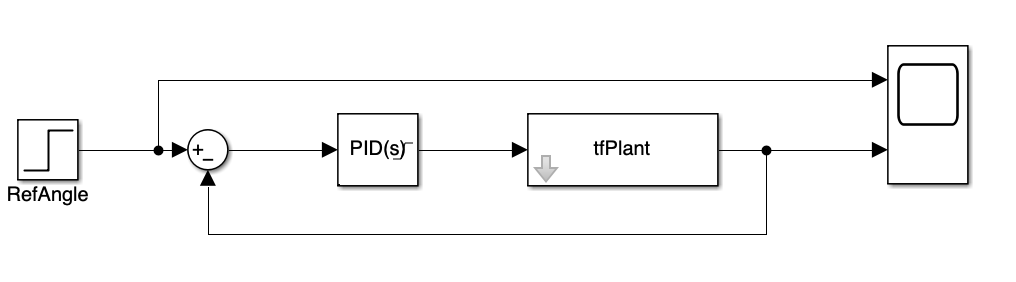
\includegraphics[width=\linewidth]{Figures/simModel.png}}
    \caption{Simulink Model for the Bot}
\end{figure}
The step responses of the system under filter coefficient N = 50 and N = 25 were
simulated to evaluate the performance of the robot under best- and worst-case
scenarios:
\begin{figure}[H]
    \centerline{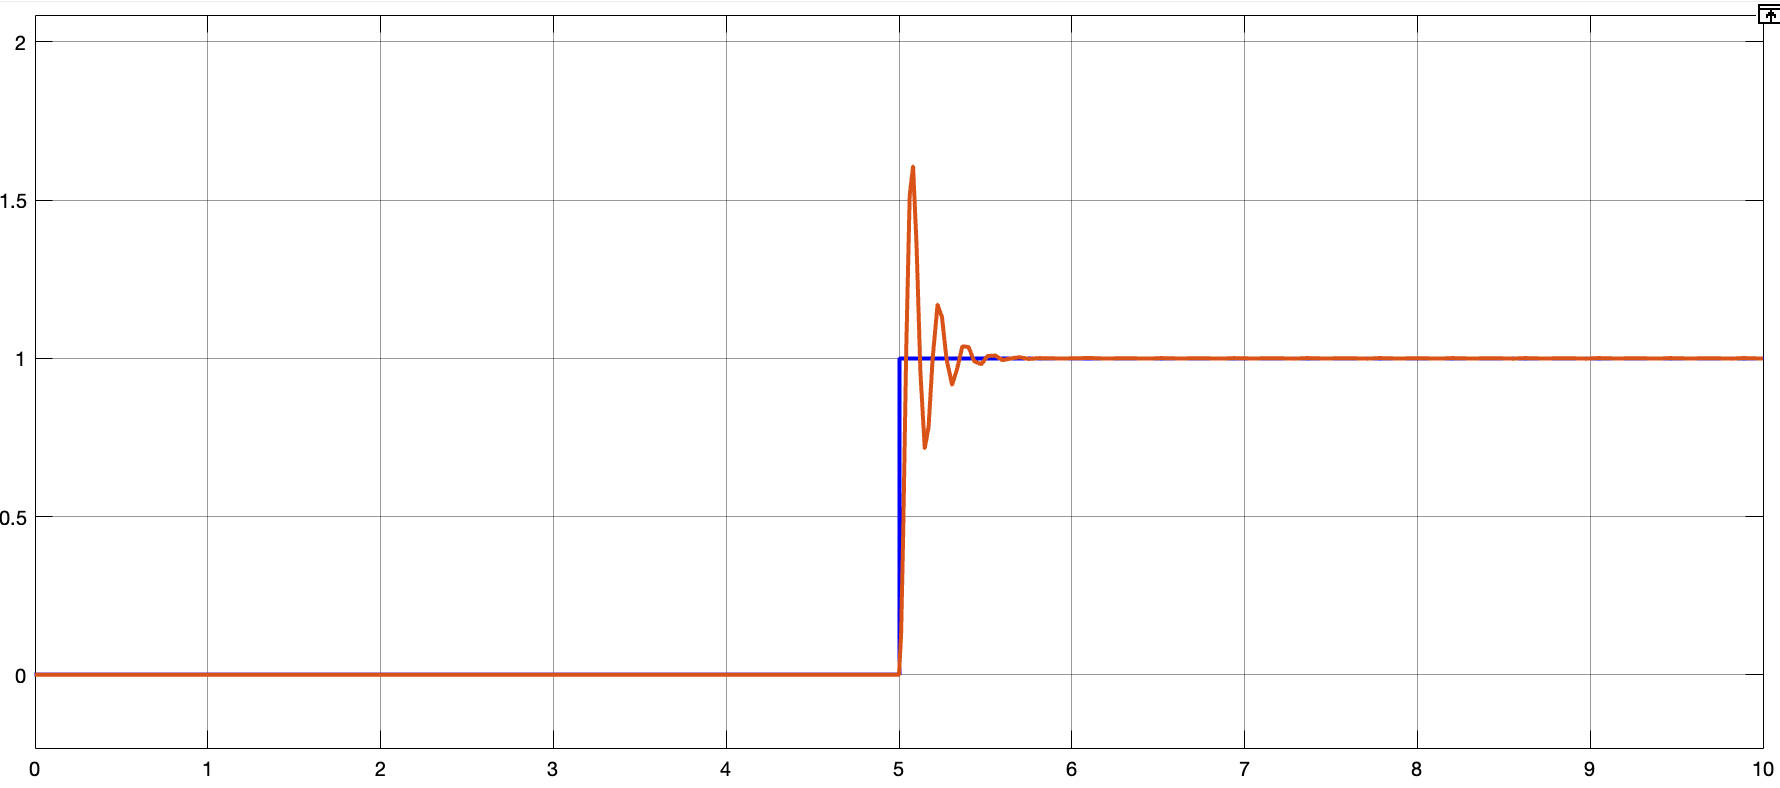
\includegraphics[width=\linewidth]{Figures/step25.png}}
    \caption{Step Response of the System with N = 25}
\end{figure}
\begin{figure}[H]
    \centerline{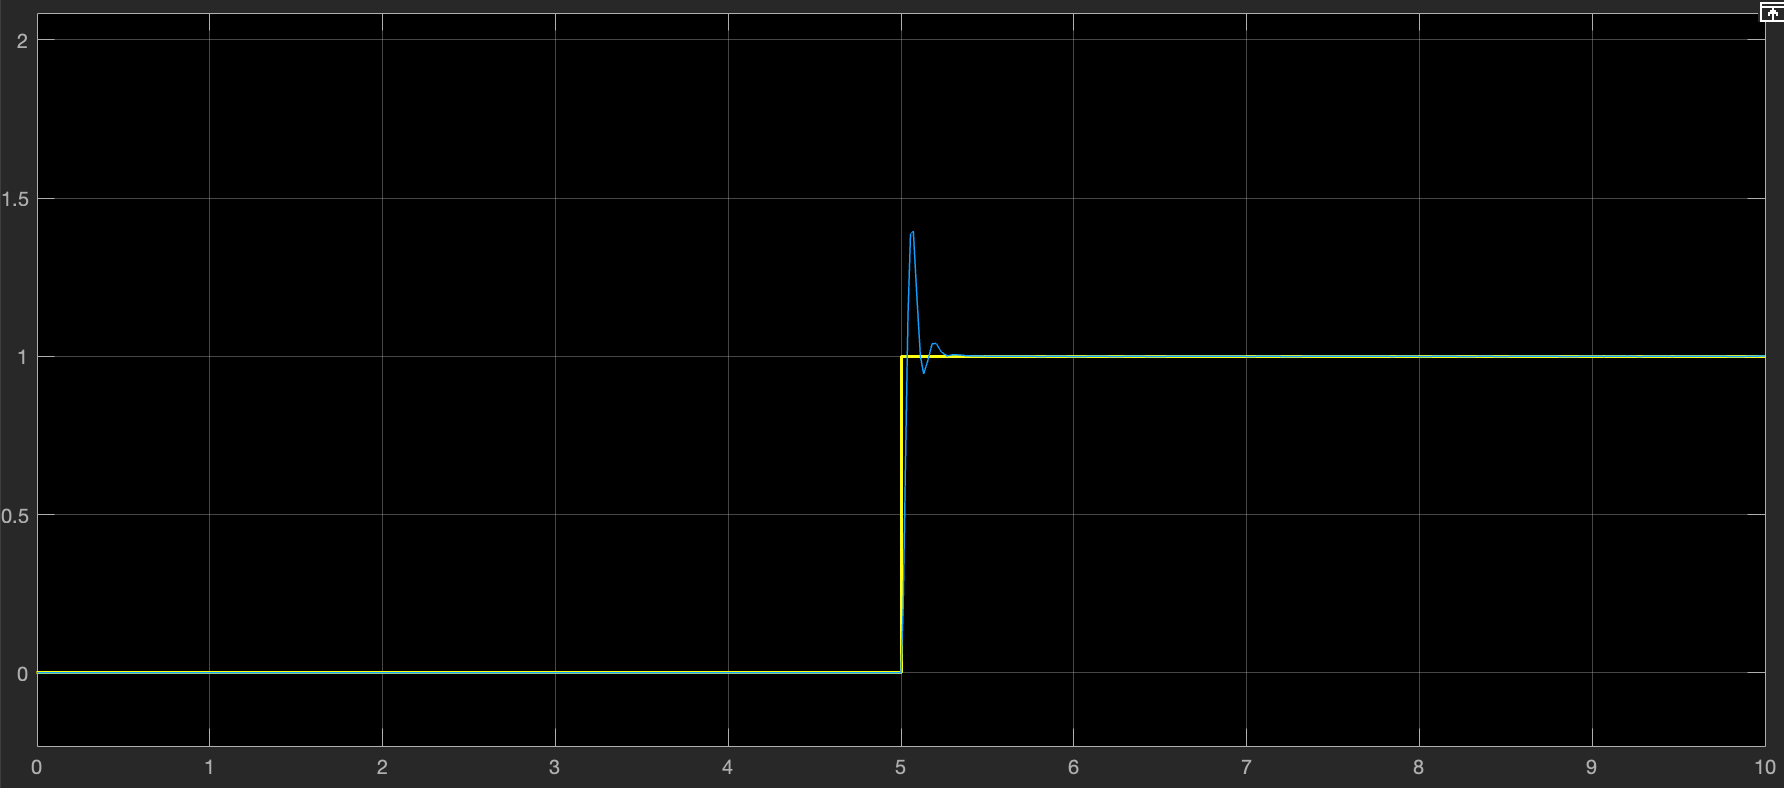
\includegraphics[width=\linewidth]{Figures/step50.png}}
    \caption{Step Response of the System with N = 50}
\end{figure}
We can see that for both cases the system is stable, with different degree of
overshoot. This implies that the design of the PID controller is effective.

\subsection{Arduino Nano 33 BLE Sense Rev2}

\begin{figure}[H]
    \centering
    \includegraphics[width=0.3\textwidth]{Figures/arduino.jpg} % Adjust width as needed
    \caption{Arduino Nano 33 BLE Sense Rev2}
    \label{fig:arduino}
\end{figure}

\begin{minipage}{\linewidth}
    The \textbf{Arduino Nano 33 BLE Sense Rev2}  is a compact and powerful microcontroller board
    designed for low-power applications. It features the Nordic \textbf{nRF52840} chipset,
    which supports \textbf{BLE} communication, includes a range of built-in sensors,
    including a 9-axis IMU (accelerometer, gyroscope, and magnetometer).
    These integrated features make it well-suited for IoT, sensor-based applications, and portable devices. \\

    This made it the ideal choice for our self-balancing robot project and was responsible for many of the core features.
    It integrated key core components in this project, particularly the \textbf{IMU} and the \textbf{BLE} module. \\
\end{minipage}


\subsubsection{Arduino IDE}

\begin{minipage}{\linewidth}
    The \textbf{Arduino IDE} was integral in quickly testing new firmware changes to the board with built-in compilation and flashing tools.
    The extensive library support significantly streamlined the development process, reducing the need for bare metal programming and allowing us to focus on the functionality.
\end{minipage}

\subsubsection{IMU Angle Measurement}
\label{sec:angle}

\begin{figure}[H]
    \centering
    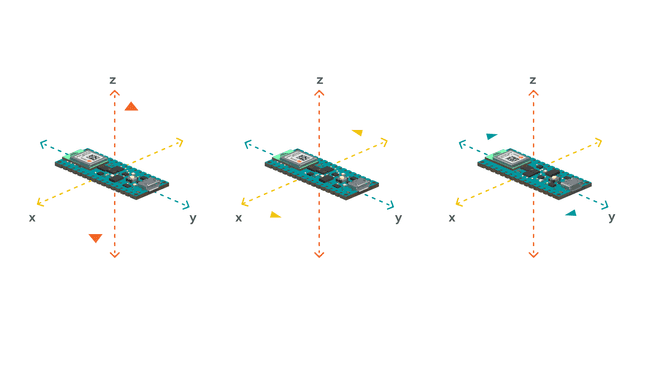
\includegraphics[width=0.6\textwidth]{Figures/imu.png} % Adjust width as needed
    \caption{IMU}
    \label{fig:imu}
\end{figure}

\begin{minipage}{\linewidth}
    The \textbf{Inertial Measurement Unit (IMU)} was a critical microcontroller component for measuring velocity, orientation, and
    gravitational forces. This enabled the tracking of motion and orientation of the \textbf{Arduino} in three-dimensional space. \\

    We used the accelerometer to measure linear acceleration and the gyroscope to monitor rotational
    movement. Both of these sensors had advantages and disadvantages, as shown in Table~\ref{tab:imu_sensors}.
    By combining them, we ensured reliable and accurate angle measurements for optimized balancing in the control feedback loop.
\end{minipage}

\subsubsection{Complementary Filter}

% \begin{figure}[H]
%     \centering
%     \includegraphics[width=0.6\textwidth]{Figures/complementary_filter.png} % Adjust width as needed
%     \caption{Complementary Filter Feedback Diagram}
%     \label{fig:complementary_filter}
% \end{figure}

\begin{minipage}{\linewidth}
    The solution to combine the strengths of both sensors was to use a complementary filter,
    which combines the accelerometer and gyroscope readings with their respective normalized weights. \\

    Since the gyroscope provided a rough estimate of the angle change, this was essential for detecting quick movements. \\
\end{minipage}

The formula used for the complementary angle is:

\[
\theta_n = k(\theta_{n-1} + \theta_{g,n}) + (1-k)\theta_{a,n},
\]

where:
\begin{itemize}
    \item $\theta_n$ is the current complementary angle,
    \item $\theta_{n-1}$ is the previous complementary angle,
    \item $\theta_{g,n}$ is the current gyroscope angle,
    \item $\theta_{a,n}$ is the current accelerometer angle,
    \item $k$ is the normalized weight.
\end{itemize}

\begin{center}
    $\therefore$ From extensive testing, a value of $k = 0.95$ was selected. \\
\end{center}

\textit{
    Lower values of $k$ caused the noise from the accelerometer to become significant, leading to large oscillations and loss of balance.
    Similarly, increasing $k$ was avoided. The gyroscope bias would accumulate quickly (i.e., without a reference point)
    and cause the robot to lose balance.
}\vspace{0.5cm}

The code snippet for this exact implementation is demonstrated in Listing \ref{lst:arduino_angle_code}.

\subsection{Autonomous-Balancing}

\begin{minipage}{\linewidth}
    The most challenging part of this project was to implement the PID controller to balance the robot. Since we had closed-loop control,
    with the measured angle acting as feedback, it was crticial that we were able to act upon new measurements when determining the control signal. \\

    Initially, we attempted to implement these \textbf{Interrupt Service Routine (ISR)} to meet a designed control frequency of $20$ Hz.
    However, this proved to accumulate complications in firmware logic and was not able to provide the expected results. \\

    We ultimately designed a control loop, run in the main program. This followed the sequence shown in Figure~\ref{fig:control_loop_diagram}.
\end{minipage}

\begin{figure}[H]
    \centering
    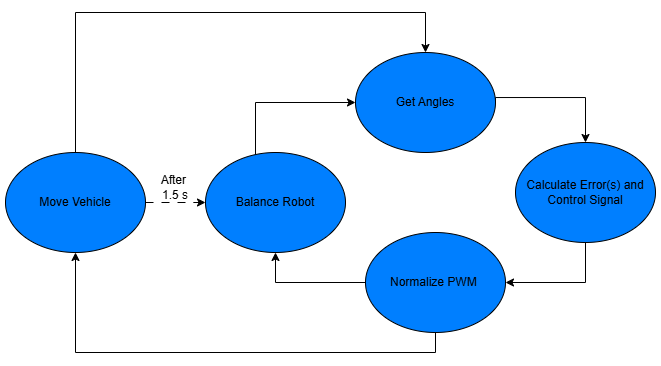
\includegraphics[width=0.75\textwidth]{Figures/Control_Loop_Diagram.png}
    \caption{Control Loop Diagram}
    \label{fig:control_loop_diagram}
\end{figure}

\begin{minipage}{\linewidth}
    This ensured that we were able to inject \textbf{PWM} signals to both motors, without the constraints typical of an \textbf{ISR}. At the same time,
    this ensured that the robot was acting upon the most recent measurements. \\

    The sign of the control signal determined whether to move the robot forward / backward to maintain balance. \\

    The source code for this implementation is shown in Listing \ref{lst:arduino_pid_code}, in the Appendix.
\end{minipage}

\subsubsection{Motor Control}

\begin{minipage}{\linewidth}
    To operate the robot wheels, we used the \textbf{DRV8833} motor driver to operate the robot with slow decay \textbf{PWM}.
    This entailed one of the motor terminals being driven to logic high, while the other was supplied the PWM signal. \\
\end{minipage}

\begin{figure}[H]
    \centering
    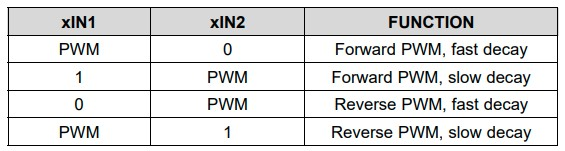
\includegraphics[width=0.5\textwidth]{Figures/PWM_Control.jpg}
    \caption{DRV8833 PWM Control}
    \label{fig:drv8833}
\end{figure}

\begin{minipage}{\linewidth}
    Supplying slow decay \textbf{PWM} enables the robot to gradually diminish its response to error angles, rather than abruptly stopping the motors.
    This was integral in ensuring the overall system behavior was stable and able to keep the robot balancing.

    \

    The source code for this implementation is shown in Listing \ref{lst:arduino_pwm_code}, in the Appendix.
\end{minipage}

\subsection{Movement}
\label{sec:movement}

\begin{minipage}{\linewidth}
    The robot was designed to move in four directions: \textbf{FORWARD, BACKWARD, LEFT, RIGHT}.
    As shown in Figure~\ref{fig:control_loop_diagram}, this was designed to be integrated into the control loop.  \\

    Balancing was the highest priority of the system at any given time. To move the robot, we injected noise into the system for a short period of time
    (i.e. $1.5$ seconds). After this, we returned to idle balancing to prevent the system from reaching a point of instability.

    \

    For the complete code snippet of this implementation, it can be found in Listing \ref{lst:arduino_movement_code}, in the Appendix.
\end{minipage}

\subsubsection{Forward/Backward Movement}

\begin{minipage}{\linewidth}
    The logic for moving the robot forward and backward was very simple. It was a matter of adjusting the setpoint angle on either side of the "zero point".
    This induced movement in the indended direction (without sacrificing balance). \\
\end{minipage}

\subsubsection{Left/Right Movement}

\begin{minipage}{\linewidth}
    The logic for moving the robot left and right was slightly more complicated and involved
    software logic to interchangeable turn and balance the robot. This can be summarized as follows: \\
\end{minipage}

\begin{itemize}
    \item \texttt{After (every) 3 iterations} of control loop : \texttt{balance robot}
    \item \texttt{If error angle $>$ allowable threshold} (i.e. $0.8^\circ$): \texttt{balance robot}
    \item Otherwise:
    \begin{itemize}
        \item To turn left: move left motor $CW$ and right motor $CCW$, with \textbf{PWM} adjusted by scale factor $0.6$
        \item To turn right: move left motor $CCW$ and right motor $CW$,  with \textbf{PWM} adjusted by scale factor $0.5$
    \end{itemize}
\end{itemize}

\subsection{Bluetooth Control}

\begin{minipage}{\linewidth}
    The robot was controlled via the \textbf{Arduino's} \textbf{Bluetooth Low Energy (BLE)} capabilities.
    The firmware was developed such that new connections need to be authorized by successfully transmitting
    the correct pairing code. This follows the workflow shown in Figure~\ref{fig:functional_diagram}. \\

    In order to send movement commands, the connection and authentication process must be successfully complete to ensure secure access. A key
    part of this process was to provide the expected pairing code to the microcontroller. \\
\end{minipage}

\begin{figure}[H]
    \centering
    \fbox{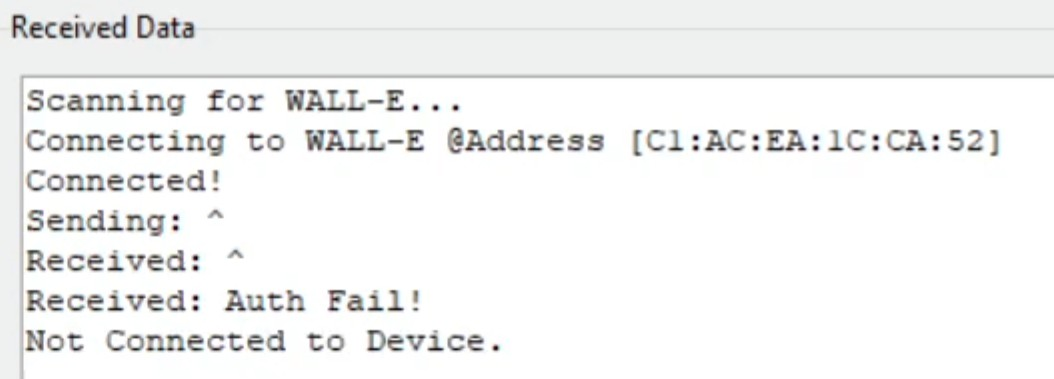
\includegraphics[width=0.5\textwidth]{Figures/Unauthorized_Connection.jpg}}
    \caption{Unauthorized Bluetooth Connection}
    \label{fig:bluetooth_unauthorized}
\end{figure}

\begin{minipage}{\linewidth}
    If unsuccesful, the robot would immediately disconnect and await an authorized user as shown in Figure~\ref{fig:bluetooth_unauthorized}. \\

    The firmware is also designed such that movement commands are placed on a lower priority. Since \textbf{BLE} can be computationally expensive,
    we polled for new commands every $100$ ms in the main loop. This was done to ensure that the control functionality is placed at highest priority,
    and we can account for the infrequent nature of user driven commands.
\end{minipage}

\subsubsection{Robot Driver App}

\begin{minipage}{\linewidth}
    We developed a \textbf{Flask} application, which used \texttt{GET/POST} request \textbf{HTTP} methods
    to asynchronously request device information from the \textbf{HTML DOM} elements and send commands to the
    \textbf{Arduino} microcontroller. \\

    This application was run from our computer and temporarily hosted to the Internet using the \textbf{ngrok} tool.
    This enabled us to access the robot via public URL from other devices (including smartphones).
\end{minipage}\vspace{0.5cm}

\begin{figure}[H]
    \centering
    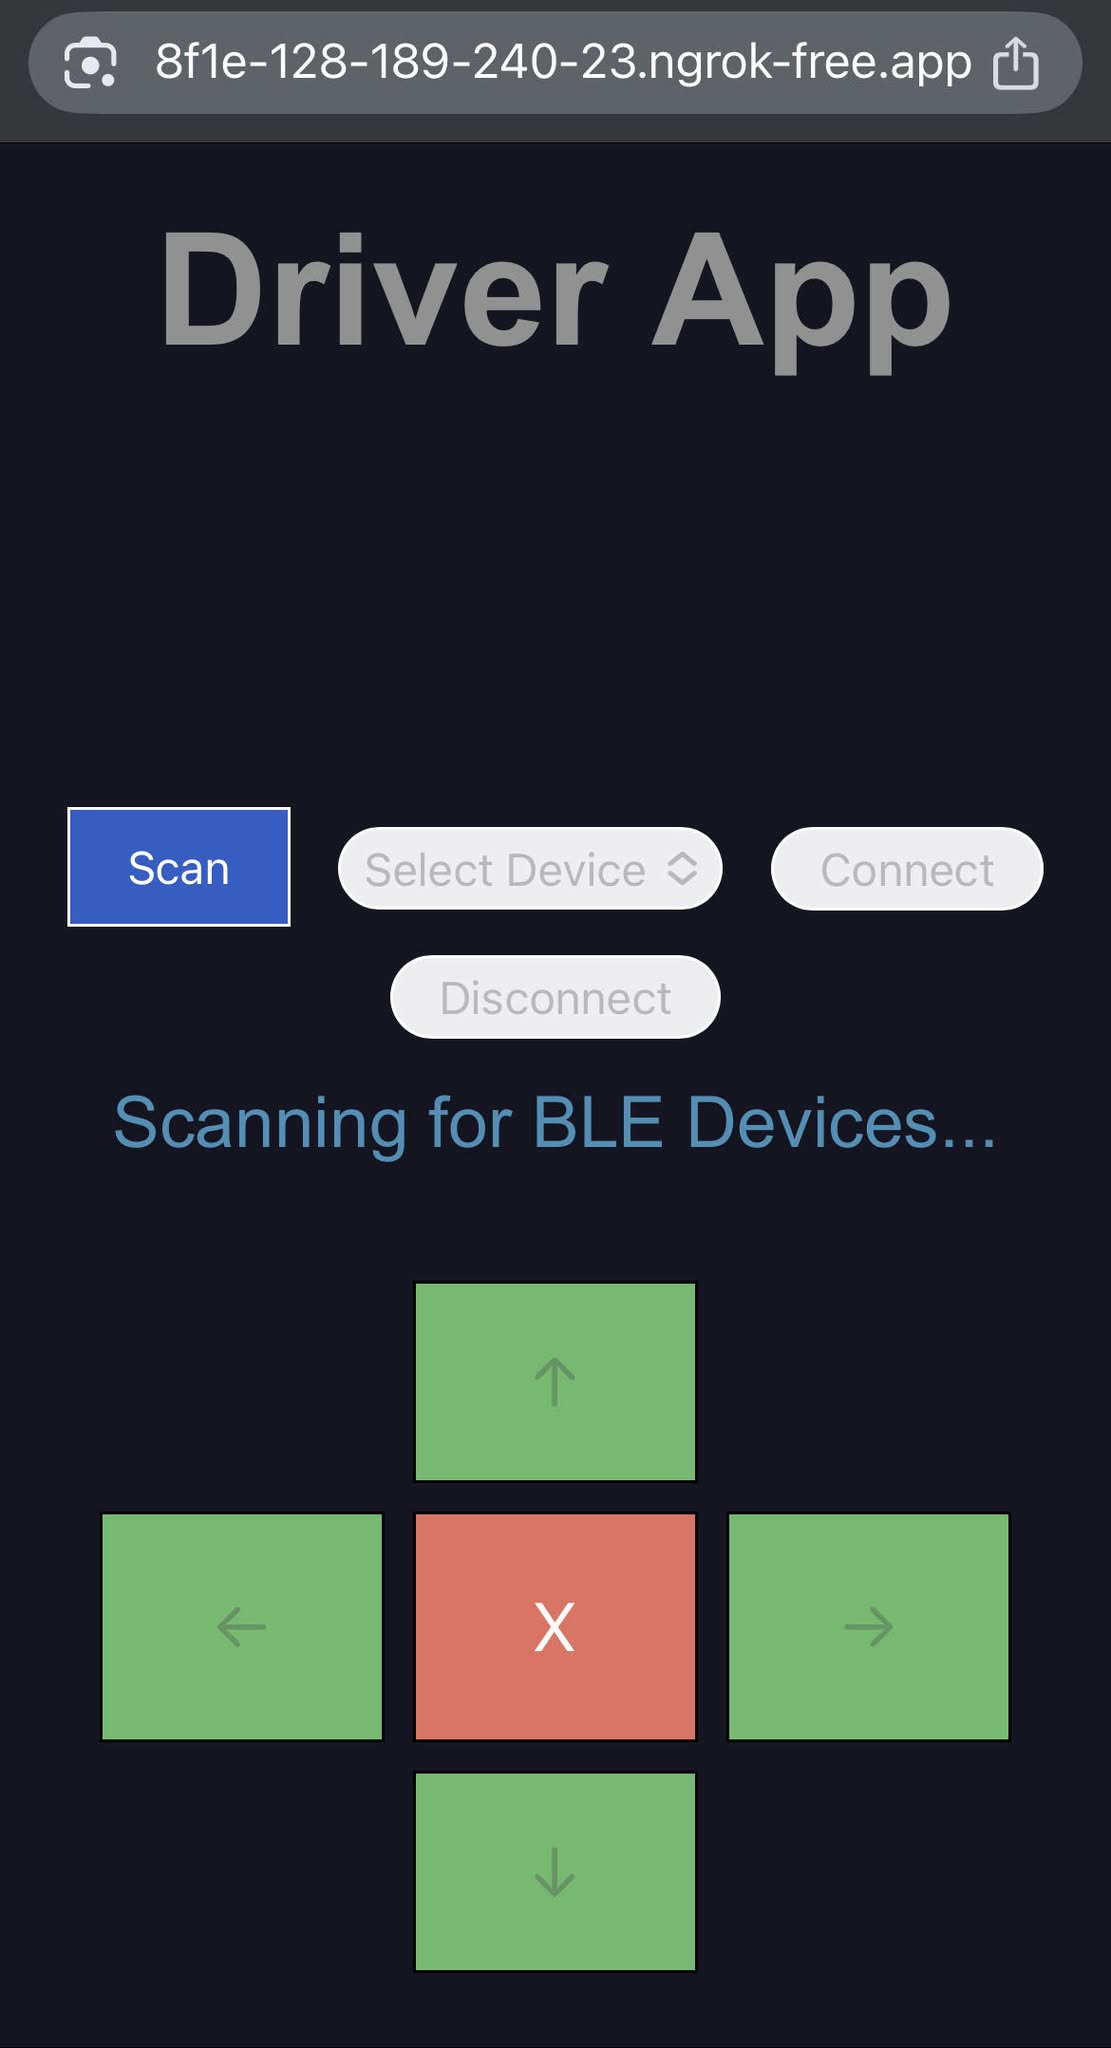
\includegraphics[width=0.25\textwidth]{Figures/Robot_Driver_App.jpg}
    \caption{Robot Driver App on iPhone 14}
    \label{fig:ble_app}
\end{figure}

\begin{minipage}{\linewidth}
    The \textbf{Flask} application had the expected pairing code programmed in the source code such that users can easily connect to and control the robot.
    We programmed the \texttt{DRIVE, LEFT, RIGHT, BACK} commands to correspond to specific bytes to be transmitted via \textbf{BLE}. \\
\end{minipage}

\begin{center}
    This is shown in the code snippet in Listing \ref{lst:driver_app_code} in the Appendix.
\end{center}

\subsection{STM32L051K8T6 Microcontroller}
\label{sec:stm32}

\begin{figure}[H]
    \centering
    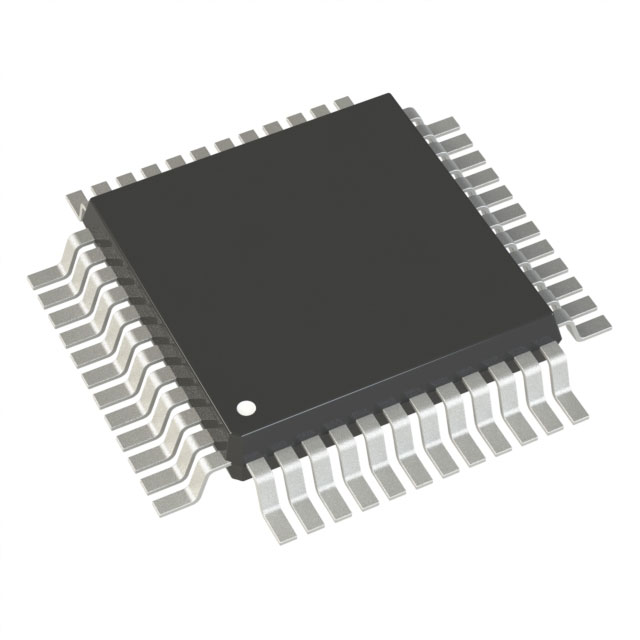
\includegraphics[width=0.3\textwidth]{Figures/stm32.jpg} % Adjust width as needed
    \caption{STM32L051K8T6 Microcontroller}
    \label{fig:stm32}
\end{figure}

The STM32L051K8T6 is a low-power microcontroller from STMicroelectronics, part of the STM32L0 series. It features an ARM Cortex-M0+ core running at up to 32 MHz, with 64 KB of flash memory and 8 KB of SRAM. For our project, this microcontroller was used to interface with the HC-SR04 (section \ref{sec:distancesensor}), TCS34725 (section \ref{sec:colorsensor}), RC522 (section \ref{sec:rfidsensor}) and the CEM-1202 (section \ref{sec:speaker}) modules. The pinout diagram is shown in Figure~\ref{fig:stm32_pinout_zoomed_in} (note that USART it was never used in the implementation).


\begin{figure}[H]
    \centering
    \begin{minipage}[b]{0.45\textwidth} % Adjust width as needed
        \centering
        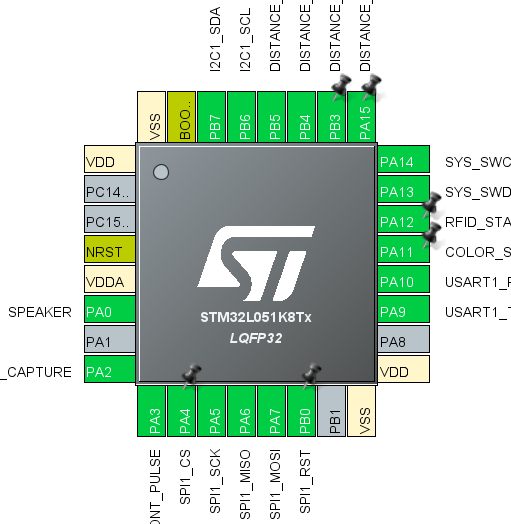
\includegraphics[width=8\textwidth, height=0.4\textheight, keepaspectratio]{Figures/stm32_pinout_in.png}
        \caption{Zoomed In Pinout}
        \label{fig:stm32_pinout_zoomed_in}
    \end{minipage} \hfill
    \begin{minipage}[b]{0.48\textwidth} % Adjust width as needed
        \centering
        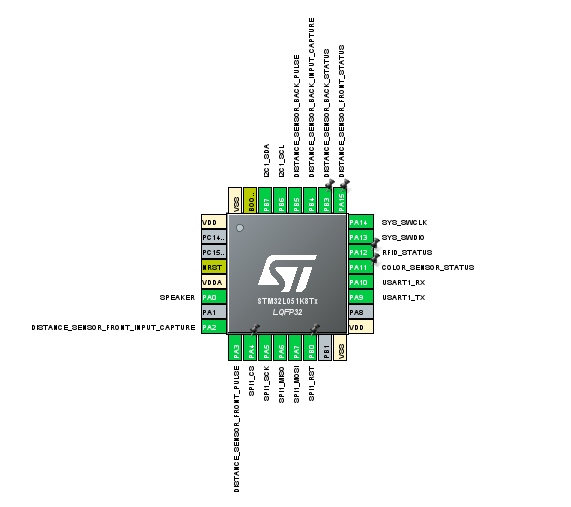
\includegraphics[width=\textwidth, height=0.4\textheight, keepaspectratio]{Figures/stm32_pinout_out.png}
        \caption{Zoomed Out Pinout}
        \label{fig:stm32_pinout_zoomed_out}
    \end{minipage}
\end{figure}

To streamline the firmware development process for the STM32, we utilized the STM32Cube IDE, provided by STMicroelectronics. This development environment facilitated faster progress by offering built-in tools and libraries, allowing us to focus on application logic rather than dealing with bare-metal programming.



\subsubsection{Distance Sensing Subsystem}
\label{sec:distancesensor}

\begin{figure}[H]
    \centering
    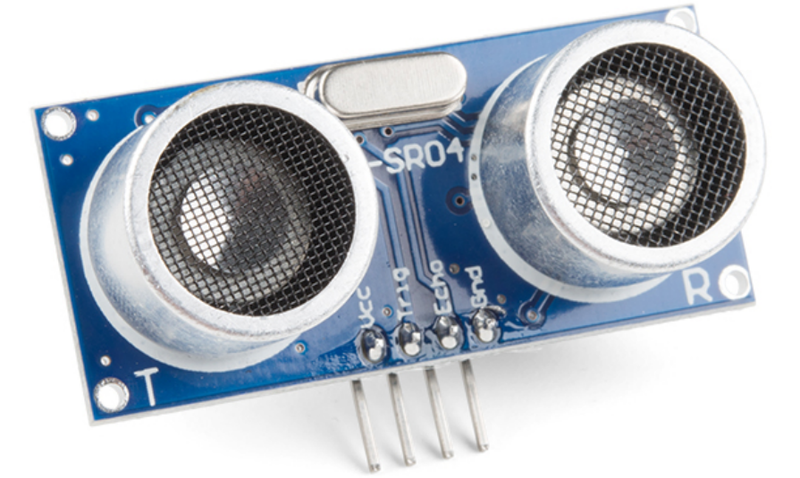
\includegraphics[width=0.3\textwidth]{Figures/distancesensor.png} % Adjust width as needed
    \caption{HC-SR04 Ultrasonic Ranging Module}
    \label{fig:distancesensor}
\end{figure}

As an extra feature, we decided to use two \textbf{HC-SR04} sensors for sensing proximity to objects. It operates by emitting an ultrasonic pulse from its transmitter and measuring the time it takes for the pulse to reflect off a nearby surface and return to the receiver. The module communicates via a simple TTL interface, requiring a 'trigger' signal to start the measurement and an 'echo' signal to indicate when the reflected pulse is received. By calculating the time interval between the trigger and echo signals, the distance to the object can be determined.

\

We decided to use timers and interrupt service routines to measure the time of this pulse. Specifically, we used the input capture mode, which would trigger on both rising and falling edges of the Echo signal, enabling precise capture of timer values at each transition. By handling these events in interrupt service routines, the CPU remained free to execute other tasks concurrently with the distance measurement process.

\

A code sample for the firmware implementation of input capture interrupt are shown in Listing \ref{lst:stm32_distancesensor_code} in the Appendix. More information about input capture mode and its implementation can be found on this site, \href{https://community.st.com/t5/stm32-mcus/how-to-use-the-input-capture-feature/ta-p/704161}{here}. If the module sensed a distance smaller than 30cm, a basic GPIO pin would be set low to communicate to the Arduino of this status.

\subsubsection{Color Sensing Subsystem}
\label{sec:colorsensor}
\begin{figure}[H]
    \centering
    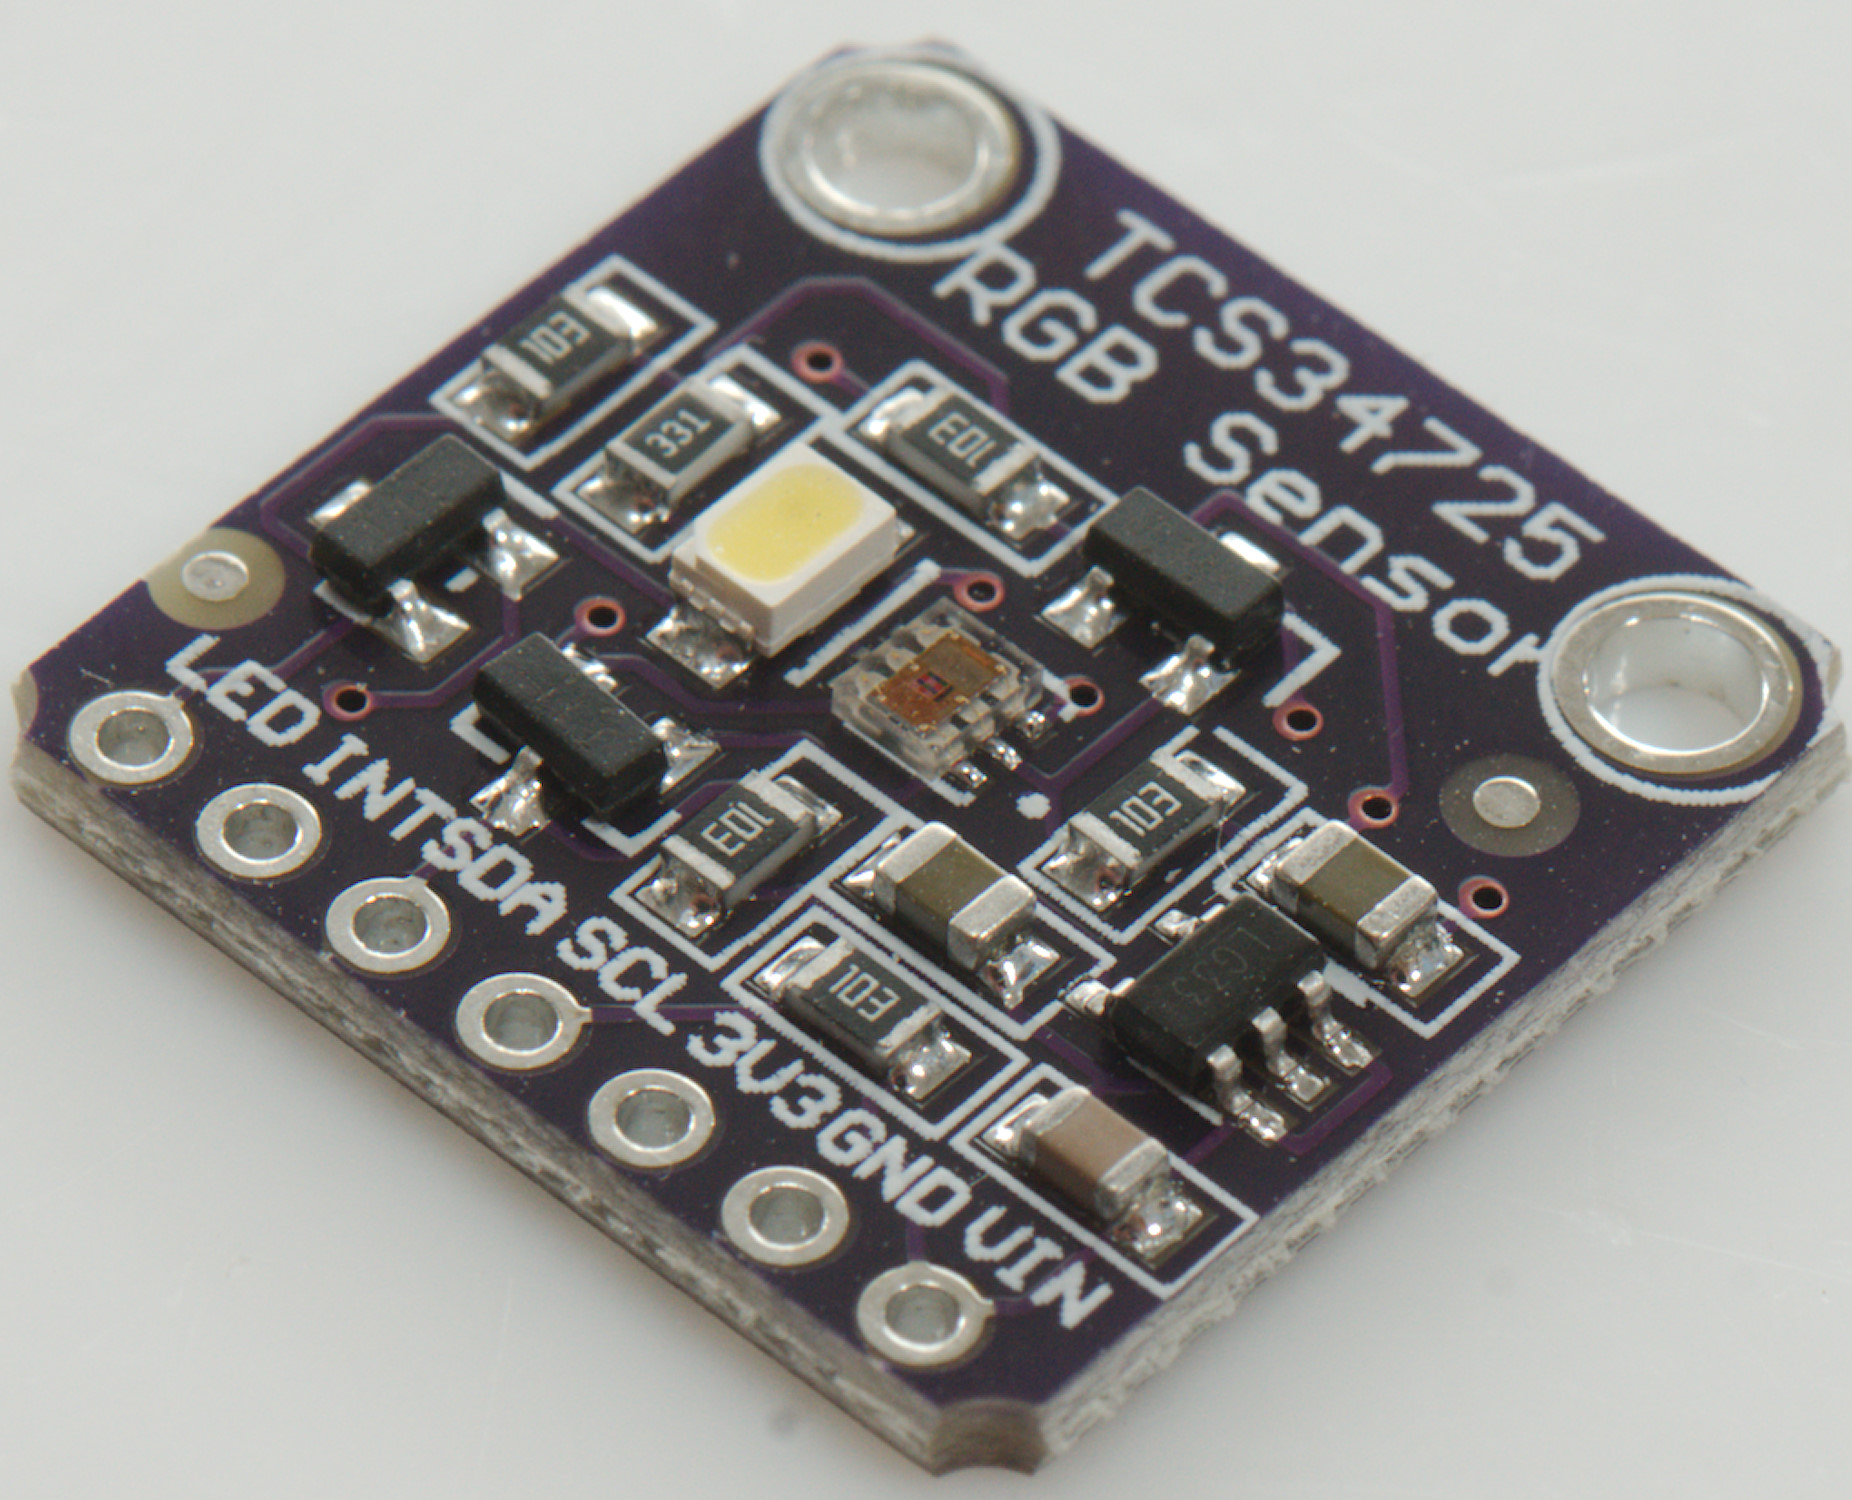
\includegraphics[width=0.3\textwidth]{Figures/colorsensor.jpg} % Adjust width as needed
    \caption{TCS34725 Light-to-Digital Sensor}
    \label{fig:colorsensor}


\end{figure}

We decided to integrate the \textbf{TCS34725} Color Sensor Module, responsible for detecting the color composition of a surface by measuring the intensity of red, green, blue, and clear light. It communicates via an I$^2$C interface, and was implemented on the \emph{STM32L051} microcontroller. The STM32 HAL libraries simplify I\textsuperscript{2}C communication, as demonstrated in Listing~\ref{lst:stm32_colorsensor_code}.

\

The \texttt{ColorSensor\_Handle} function is called within the main control loop. It reads the values from each color channel register (16 bits) and determines the most dominant color. If the red channel is the most prominent, the speaker is triggered to notify the user of the sensor's detection. When this would occur, a basic GPIO pin would be set low to communicate to the Arduino of this status.


\subsubsection{RFID Security System}
\label{sec:rfidsensor}
\begin{figure}[H]
    \centering
    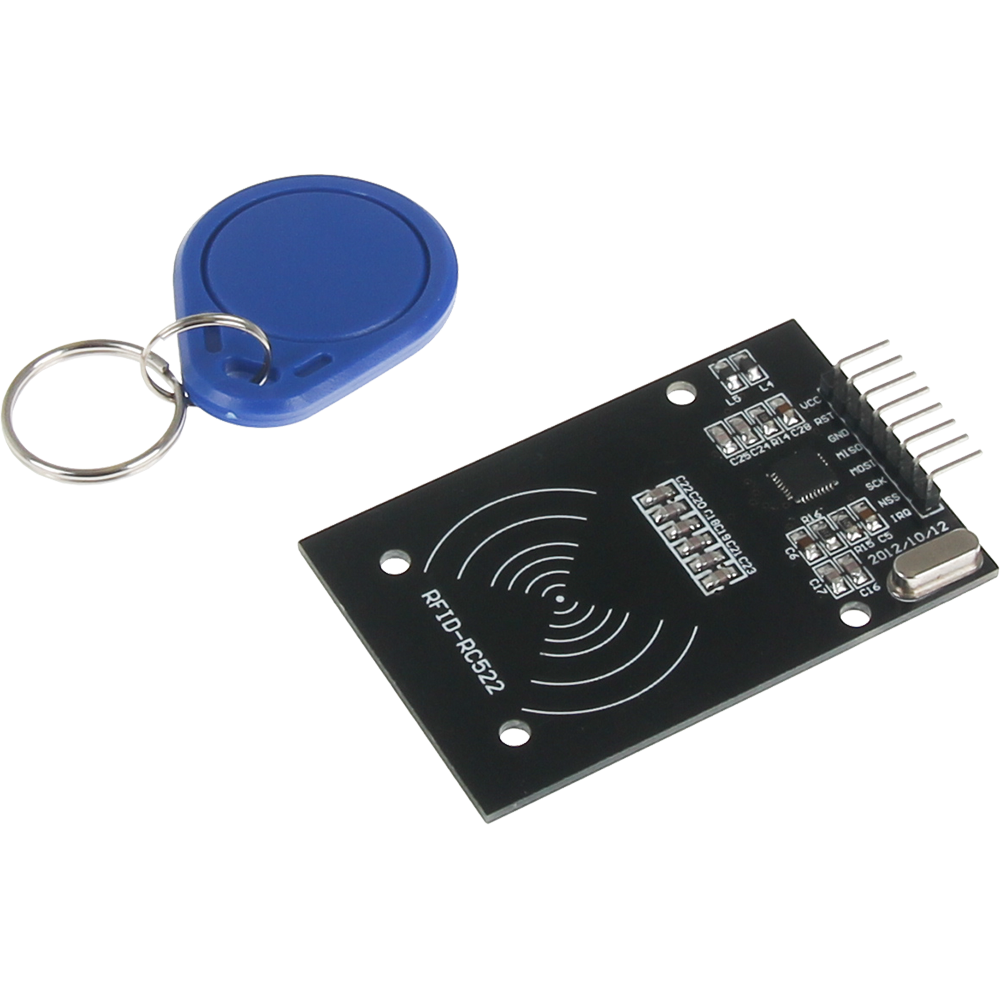
\includegraphics[width=0.3\textwidth]{Figures/rfidsensor.png} % Adjust width as needed
    \caption{RC522 Contactless Reader IC}
    \label{fig:rfidsensor}


\end{figure}

The \textbf{RC522} RFID Module was responsible for detecting and reading passive RFID tags using radio frequency communication at 13.56MHz. It operates over an SPI interface, allowing for fast and efficient data exchange with the \emph{STM32L051} microcontroller. When a tag enters the RF field generated by the module’s antenna, the RC522 initiates a handshake protocol and reads the tag’s unique identifier (UID) stored in its internal memory.

\

In the case where the correct RFID tag would be scanned, a basic GPIO pin would be set low and the speaker would be triggered to communicate to the Arduino of this status. The remaining logic specific to our application is shown in Listing \ref{lst:stm32_rfidsensor_code} in the Appendix.

\subsubsection{CEM-1302 Speaker/Buzzer}
\label{sec:speaker}
\begin{figure}[H]
    \centering
    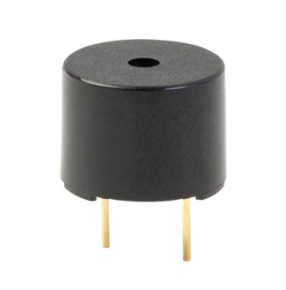
\includegraphics[width=0.2\textwidth]{Figures/speaker.png} % Adjust width as needed
    \caption{CEM-1302 Speaker/Buzzer}
    \label{fig:speaker}
\end{figure}



We used the CEM-1302 buzzer to indicate the following key events:
\begin{itemize}
    \item RFID: Indicating successful and unsuccessful RFID card scans
    \item Ultrasonic Sensor: Alerting when the distance between the robot and an object is too small
    \item Color Sensor: Signaling when the color sensor detects a predominantly red color
\end{itemize}

When any of these events occurred, the speaker would either beep, or stay on, depending on the scenario. Code for the setup can be seen in Listing \ref{lst:stm32_speaker_code}. The speaker was also developed on the \emph{STM32L051}, using a square wave PWM running at 2.048kHz. GPIO pins for these events were used to communicate with the Arduino Nano for simplicity and speed.

\subsection{Raspberry Pi Zero 2 W}

The \textbf{Raspberry Pi Zero 2 W} is an affordable single-board computer designed for
embedded systems and IoT applications. We leveraged its camera connector (CSI-2 interface)
to interface with a \textbf{Freenove 5MP Camera}, as well as its Wi-Fi capabilities to
wirelessly access it the \textbf{Raspberry Pi Connect} software.

\begin{figure}[H]
    \centering
    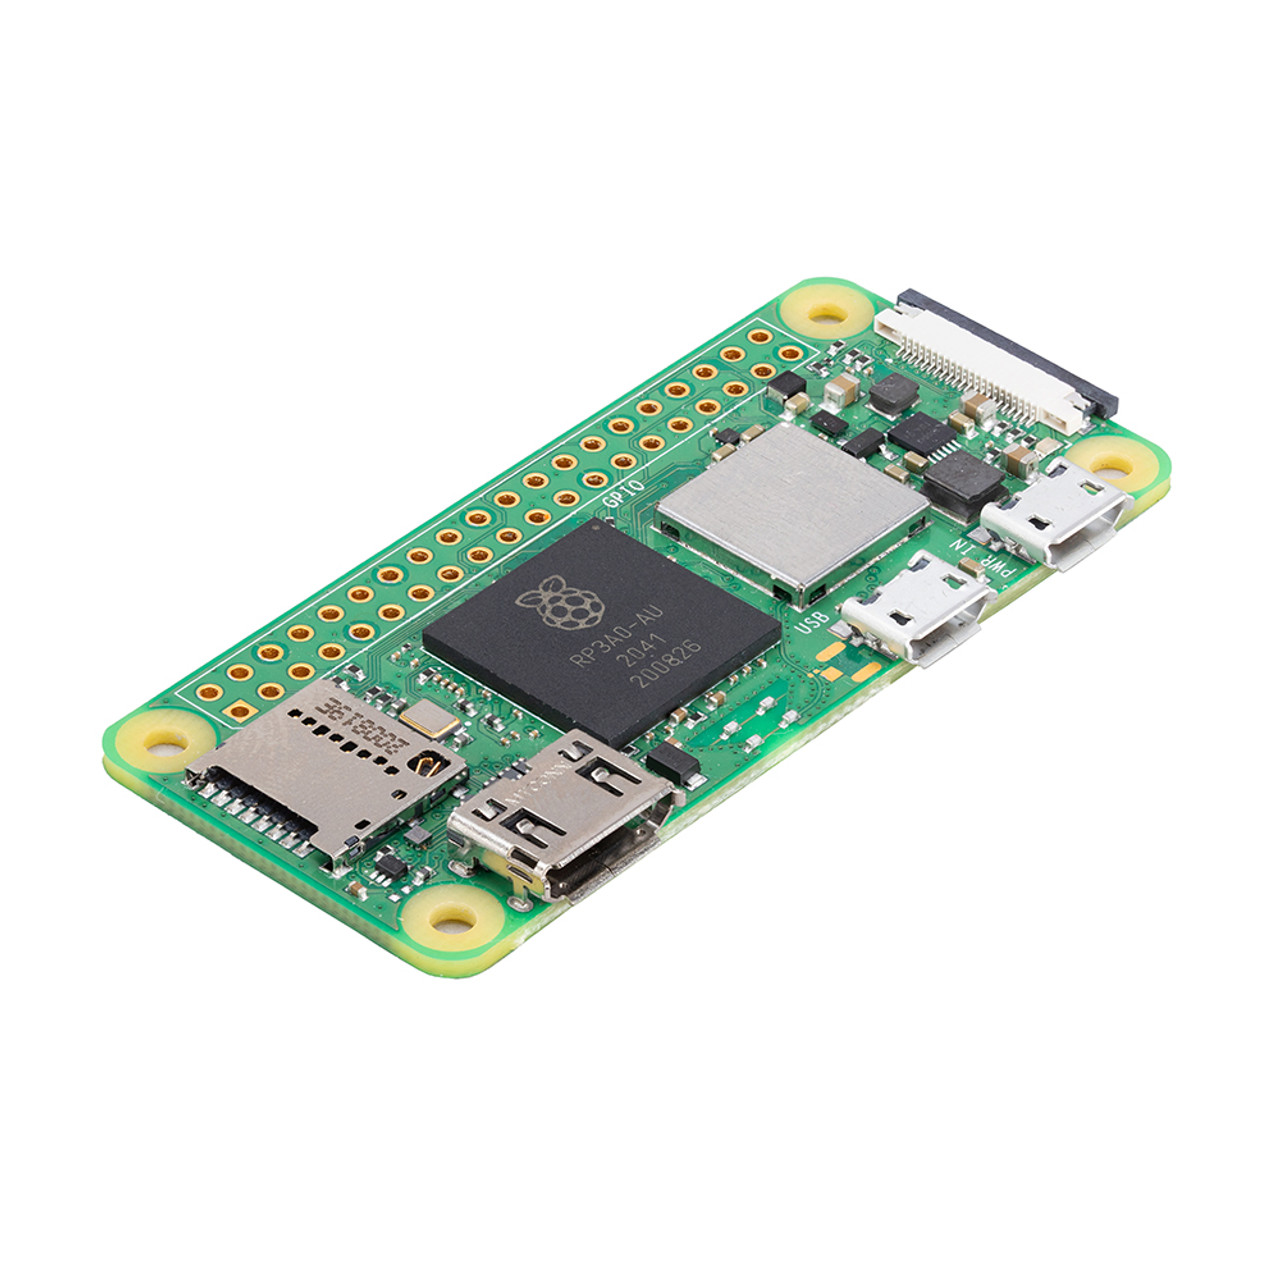
\includegraphics[width=0.3\textwidth]{Figures/PiZero_2.jpg}
    \caption{Raspberry Pi Zero 2 W}
    \label{fig:raspberrypi}
\end{figure}

\subsubsection{Camera App}

\begin{minipage}{\linewidth}
    We developed a \textbf{Python} application to display the live camera feed in a \textbf{Tkinter GUI} window,
    allowing the user to observe and record the operation of the robot. The user interface provided the ability to also
    take snapshots and store these in the \textbf{SD Card} storage. \\

    The live feed was largely a result of scheduling an update function with \textbf{Tkinter}'s \texttt{after(\dots)} method,
    which allowed us to sample camera frames at a rate of $20$ FPS. \\

    Since the \textbf{Raspberry Pi Zero 2 W} had power and performance constraints (i.e. $512$ MB of SDRAM),
    we ensured that the application was optimized for performance and iterated software versioning
    to minimize resource consumption. The camera was configured to capture frames at a resolution of $480$ pixels to account for this. \\
\end{minipage}

\begin{figure}[H]
    \centering
    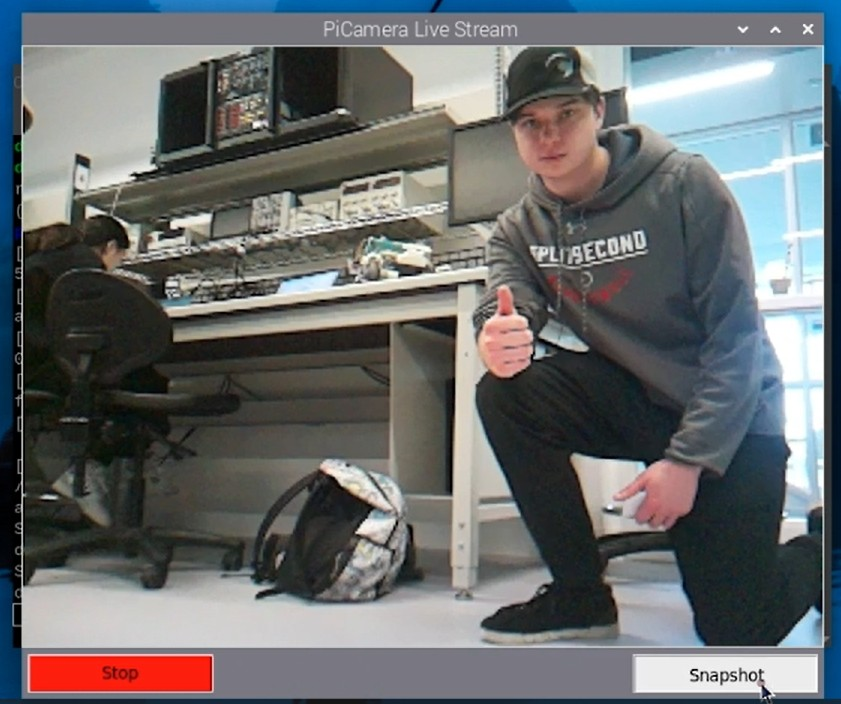
\includegraphics[width=0.5\textwidth]{Figures/PiCamera_App.jpg}
    \caption{PiCamera Application}
    \label{fig:camera_app}
\end{figure}

\begin{center}
    The class and methods for the camera display are shown in Listing \ref{lst:picamera_display_code} in the Appendix. \\
\end{center}


\begin{minipage}{\linewidth}
    Early on in development, we switched from the \textbf{Kivy} framework. This provided smoother animations, but rendering was
    hardware accelerated. We were unconfident with the \textbf{Raspberry Pi Zero 2 W}'s ability to provide adequate performance with this,
    and ported the application to the current implementation.
\end{minipage}

\subsubsection{AWS Bucket}

\begin{minipage}{\linewidth}
    Another constraint we considered during implementation was the inability to
    connect to the \textbf{Raspberry Pi} without powering on the robot. Having to access recording and snapshots
    would be quite cumbersome for the user. \\
\end{minipage}

\begin{figure}[H]
    \centering
    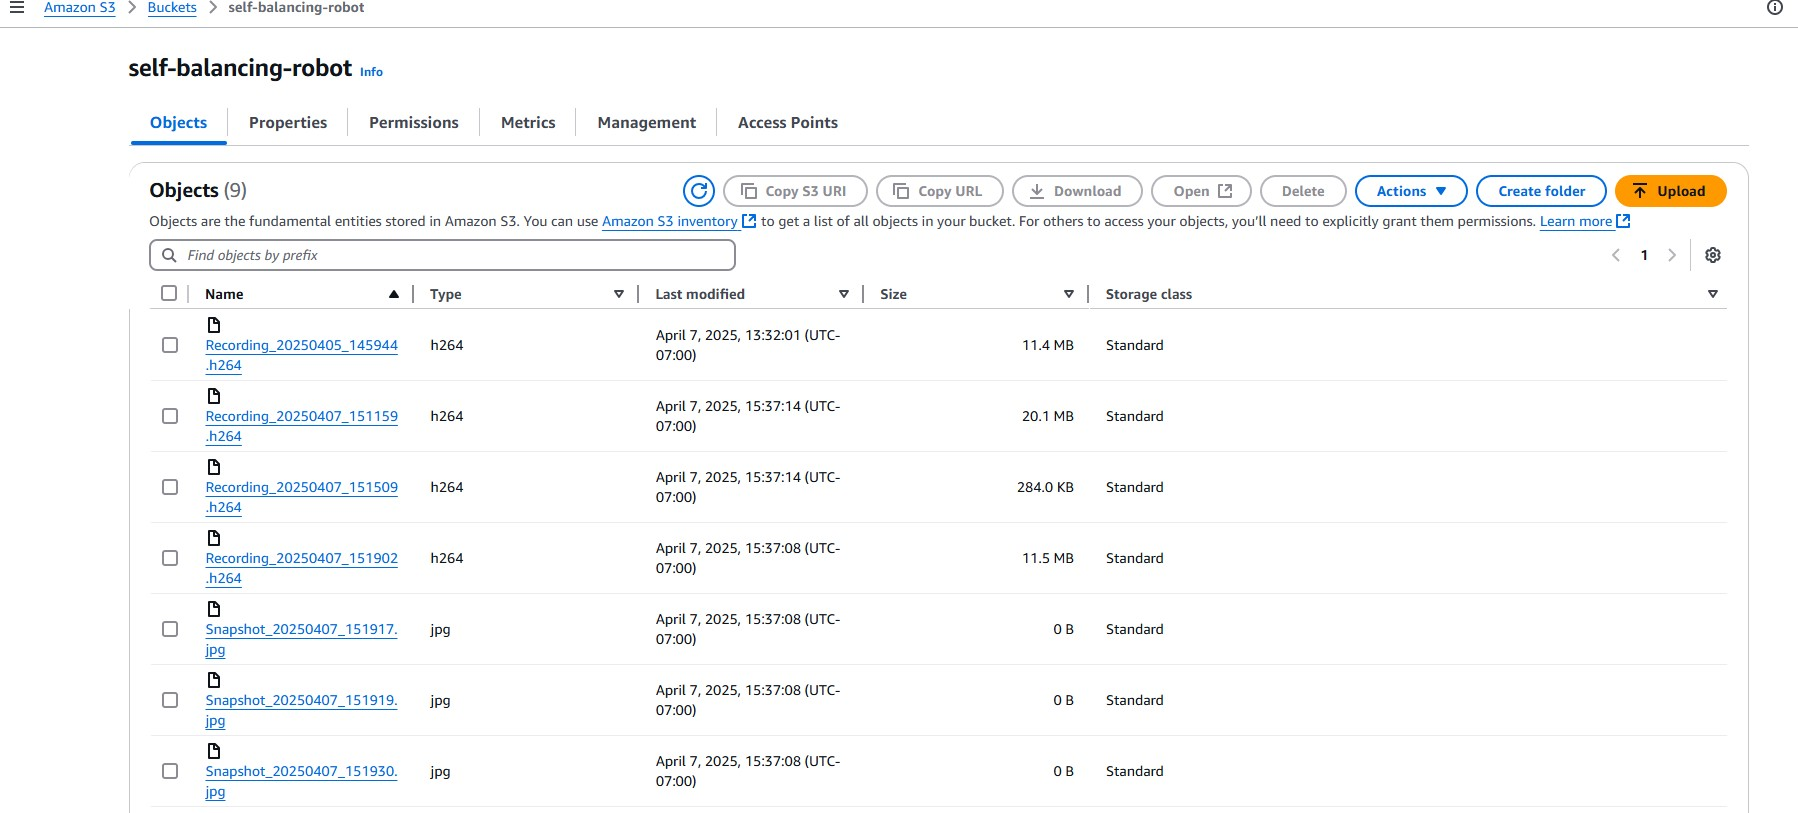
\includegraphics[width=1\textwidth]{Figures/S3Bucket_Files.jpg}
    \caption{AWS S3 Bucket}
    \label{fig:s3_bucket}
\end{figure}

\begin{minipage}{\linewidth}
    We created an \textbf{AWS S3 Bucket} and uploaded the camera recordings and snapshots during operation.
    The \textbf{Boto} package enabled us to implement this in our \textbf{Python} application by leveraging the \textbf{AWS SDK}.
    We were able to download these files from the \textbf{AWS S3 Bucket} to our local machine for offline access.
\end{minipage}

\section{Verification and Validation}
\subsection{Verification}

\begin{minipage}{\linewidth}
    To evaluate the core functionality of the robot, we leveraged the \textbf{Serial} and \textbf{BLE} capability of the \textbf{Arduino} microcontroller to both observe and modify \textbf{PID} I/O signals. \\

    This was done to compare performance as we tweaked parameters. \\
\end{minipage}

\subsubsection{Angle Measurement Accuracy}

\begin{minipage}{\linewidth}
    Early on in development, we realized that accurate angle measurements were critical to the robot's ability to successfully
    balance itself. \\

    We developed a \textbf{Python} user interface to visualize the angle measurements from the \textbf{Arduino} in real-time,
    included in Listing \ref{lst:stripchart_code} in the Appendix. \\
\end{minipage}

\begin{figure}[H]
    \centering
    \fbox{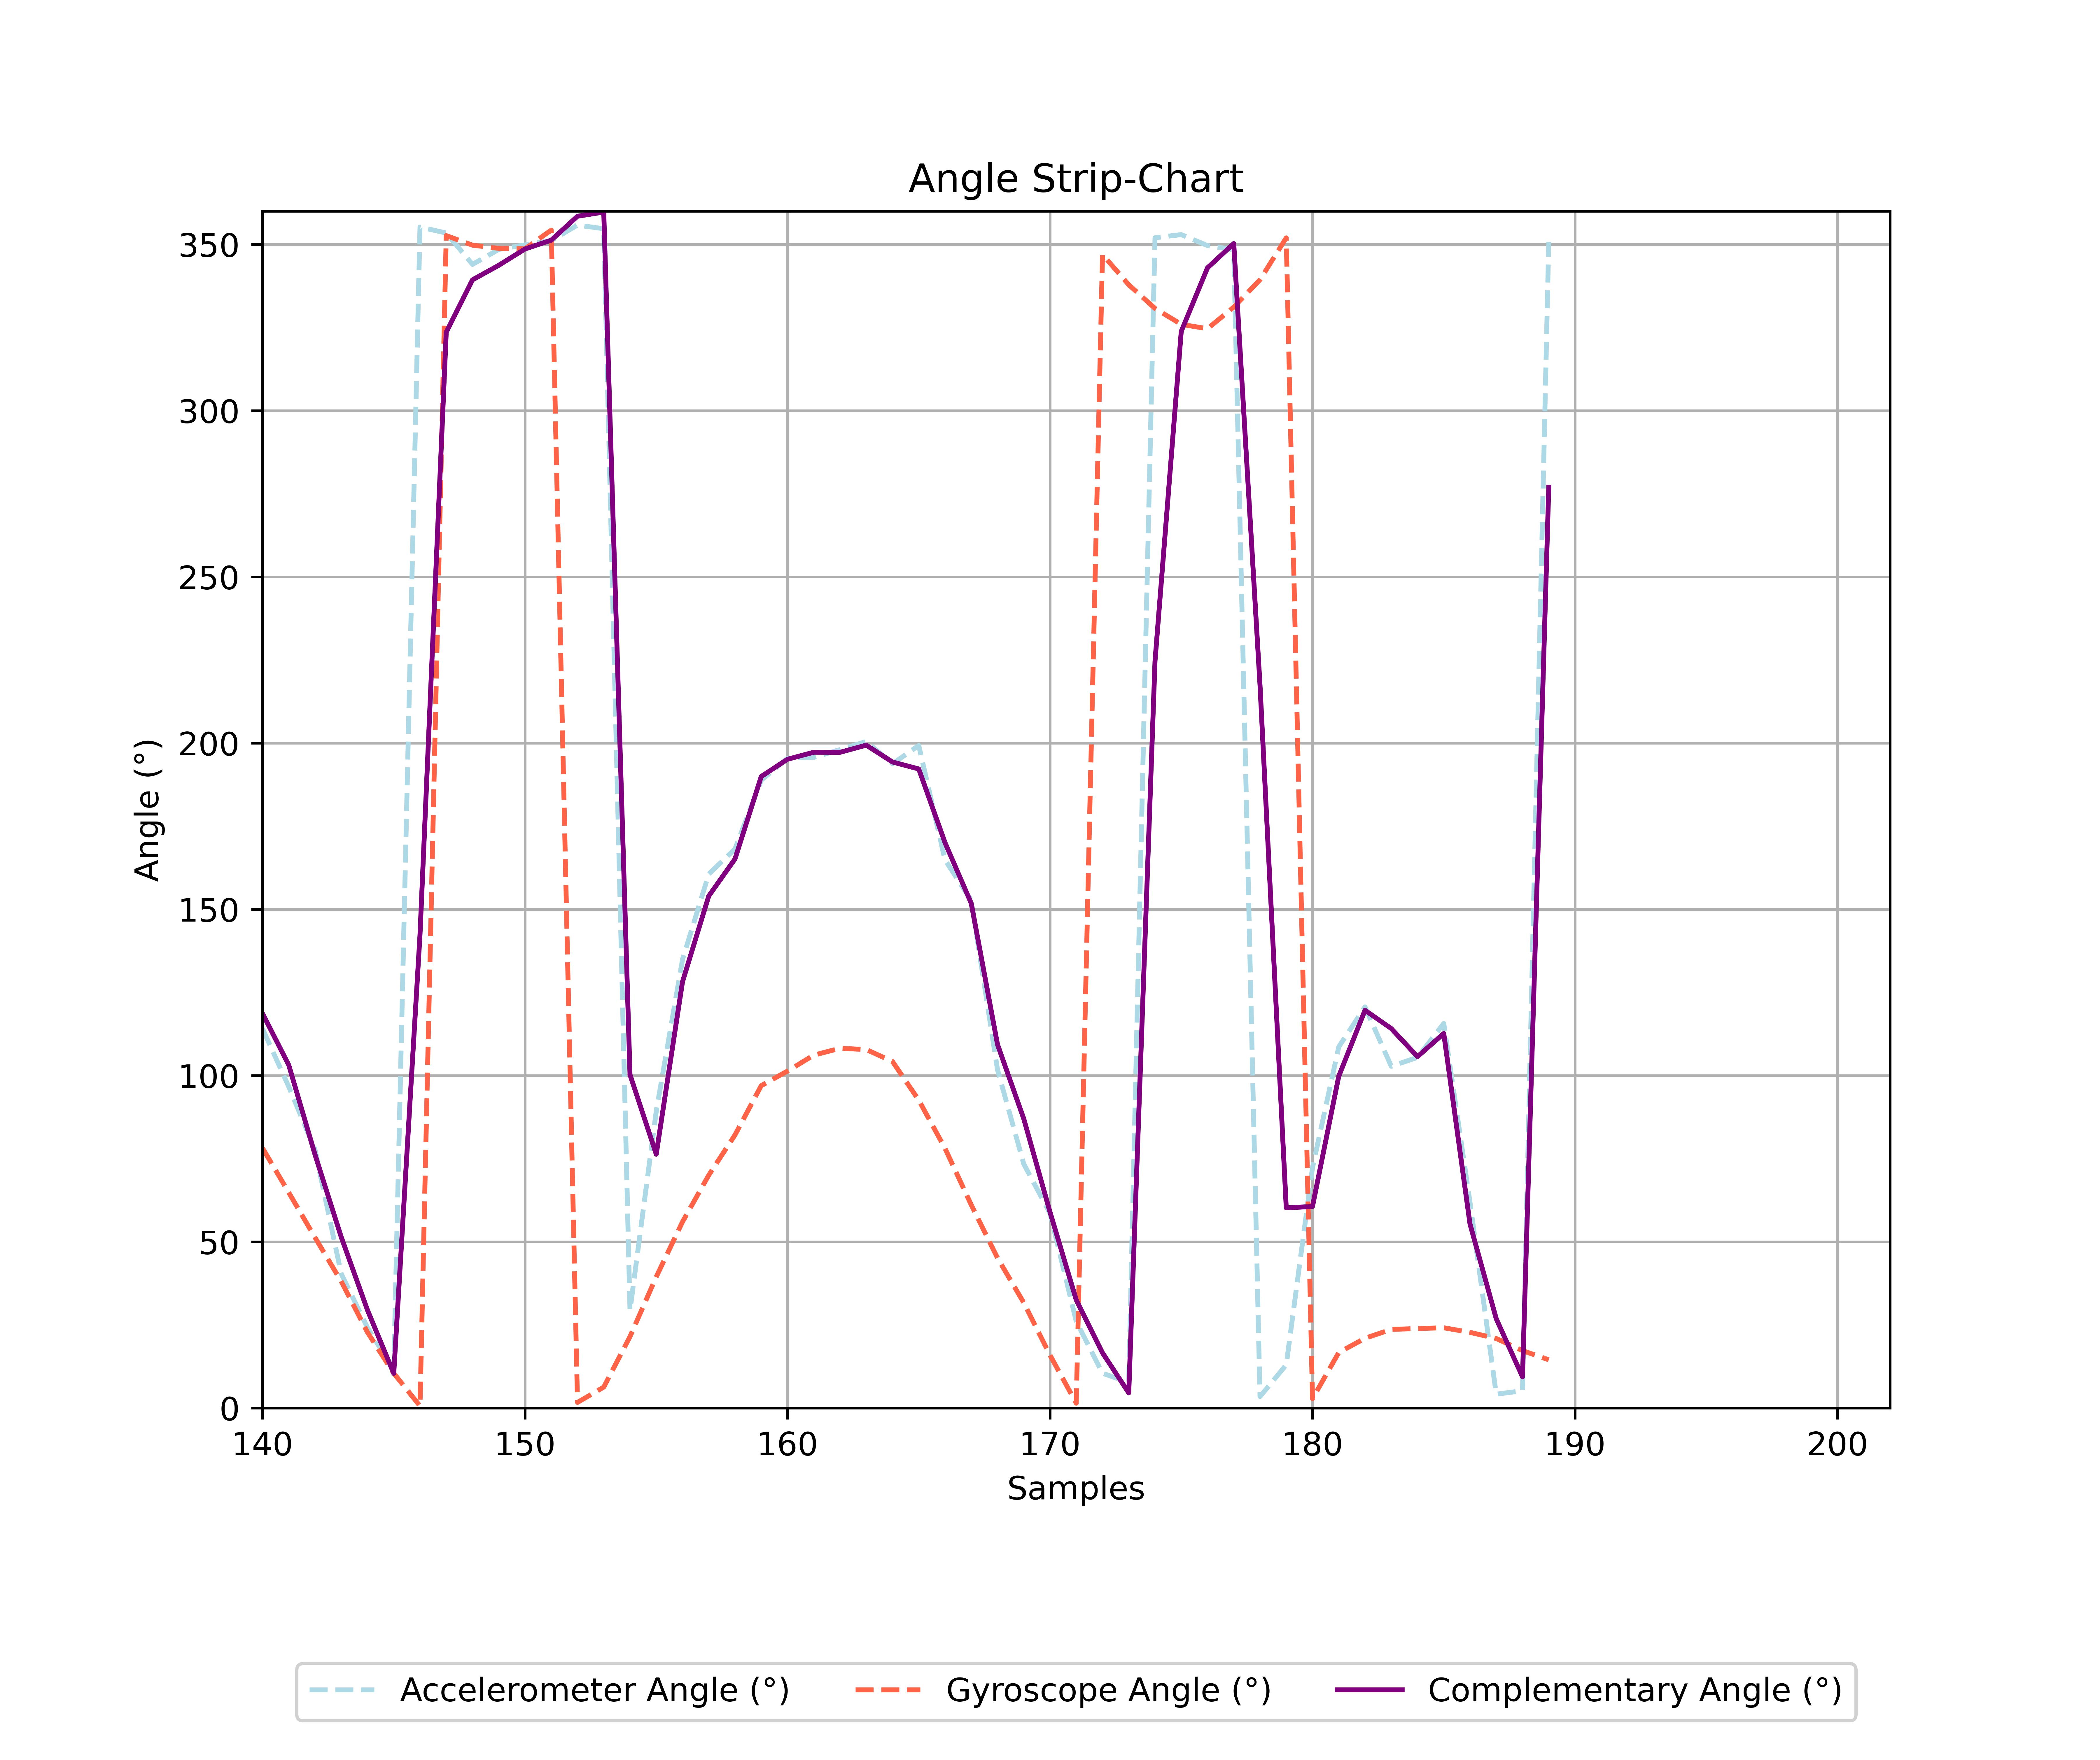
\includegraphics[width=0.6\textwidth]{Figures/Stripchart_k06.jpg}}
    \caption{Angle Measurements (k = 0.6)}
    \label{fig:stripchart_k06}
\end{figure}

\begin{minipage}{\linewidth}
    As shown in the example in Figure~\ref{fig:stripchart_k06}, we rotated the \textbf{Arduino} microcontroller within a predefined angle range
    and observed the complementary filter's performance with a given $k$ value. \\

    From saving and comparing these logs, we observed trends in the
    angle measurements from the accelerometer and gyroscope. This enabled us to optimize the benefits of both sensor and
    was critical in ensuring that we were able to balance the robot successfully.
\end{minipage}

\subsubsection{PID Tuning}

\begin{minipage}{\linewidth}
    Similarly, we developed a debugging tool in the \textbf{Arduino} firmware to tune \textbf{PID} parameters during operation.
    The source code for this is shown in Listing \ref{lst:arduino_ble_tuning_code} in the Appendix. \\
\end{minipage}

\begin{minipage}{\linewidth}
    When we were confident in the actual system level logic, we used the \textbf{BLE} capabilities to tune the following parameters. \\
\end{minipage}

\begin{itemize}
    \item PID Gains ($K_p$, $K_i$, $K_d$)
    \item Complementary Filter Weight ($k$)
    \item Setpoint Angle ($\theta_{set}$)
\end{itemize}

\begin{minipage}{\linewidth}
    During operation, we observed the effect of increasing / decreasing each of these on meeting the balancing requirements from
    Table~\ref{tab:functional_requirements}. \\
\end{minipage}

\begin{table}[H]
    \centering
    \renewcommand{\arraystretch}{1.3}
    \begin{tabularx}{\textwidth}{|c|X|X|}
        \hline
        \textbf{Parameter} & \textbf{Behavior When Increased} & \textbf{Behavior When Decreased} \\
        \hline
        $K_p$ & --- & --- \\
        \hline
        $K_i$ & --- & --- \\
        \hline
        $K_d$ & --- & --- \\
        \hline
        $k$ & Faster, Smooth Response. Accumulates Drift. & Increases Noise Influence, Experiences Jitter. No Drift. \\
        \hline
        $\theta_{set}$ & Drifting in Forward Direction. & Drifting in Backward Direction. \\
        \hline
    \end{tabularx}
    \caption{PID Parameters and System Behavior}
    \label{tab:parameter_behavior}
\end{table}

\subsection{Validation}: Testing methods and results to demonstrate that the product actually will meet the high-level goals.

\section{Conclusions and Future Work}
Summary of the outcomes achieved/learned
Recommendations for next steps or further improvements


\section{References}
Cite any academic papers, industry standards, or prior work consulted in the project. Use consistent reference
formatting (e.g. https://pitt.libguides.com/citationhelp/ieee )


\section{Appendices}
Include sections that do not fit well in the main body of the report but help to show the development progress and justify your decisions. These might include (but may not be restricted to) the following:

\subsection{Appendix: Budget}

\begin{figure}[H]
    \centering
    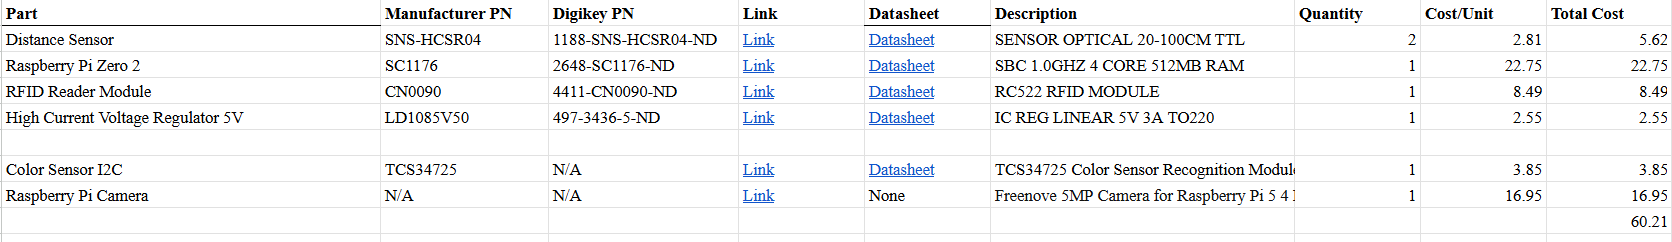
\includegraphics[width=1\textwidth]{Figures/financials.png}
    \caption{Extra Features Budget Rundown}
    \label{fig:financials}
\end{figure}

\subsection{Appendix: Technical Calculations and Simulations}

\begin{table}[H]
    \centering
    \label{tab:imu_sensors}
    \begin{tabularx}{\textwidth}{|l|X|X|}
    \hline
    \textbf{Sensor} & \textbf{Pros} & \textbf{Cons} \\
    \hline
    \textbf{Accelerometer} &
    \begin{itemize}
        \item accurate gravitational readings
        \item zero-mean noise
    \end{itemize} &
    \begin{itemize}
        \item high noise variance (especially with motor vibrations)
    \end{itemize} \\
    \hline
    \textbf{Gyroscope} &
    \begin{itemize}
        \item lower noise over short time periods
    \end{itemize} &
    \begin{itemize}
        \item accumulates bias over time
    \end{itemize} \\
    \hline
    \end{tabularx}
    \caption{IMU Sensors: Pros and Cons}
\end{table}

\subsection{Appendix: Drawings, Schematics, and Blueprints}

\subsection{Appendix: Datasheets / Product Specifications}
Supporting Datasheets and Technical Documentation for Core Features (does not include battery related components, mechanical components, or generic electrical components):

\begin{enumerate}
    \item \href{https://docs.arduino.cc/resources/datasheets/ABX00069-datasheet.pdf}{Arduino Nano 33 IoT (ABX00069) Datasheet}
    \item \href{https://www.pololu.com/file/0J1736/pololu-37d-metal-gearmotors-rev-1-2.pdf}{Pololu 37D Metal Gearmotor Specifications}
    \item \href{https://www.ti.com/lit/ds/symlink/drv8833.pdf?ts=1743785858420}{Texas Instruments DRV8833 Dual H-Bridge Motor Driver Datasheet}
\end{enumerate}

\

Supporting Datasheets and Technical Documentation for Additional Features:
\begin{enumerate}
    \item \href{https://cdn.sparkfun.com/datasheets/Sensors/Proximity/HCSR04.pdf}{HC-SR04 Ultrasonic Distance Sensor}
    \item \href{https://cdn-shop.adafruit.com/datasheets/TCS34725.pdf}{TCS34725 Color Sensor}
    \item \href{https://datasheets.raspberrypi.com/rpizero2/raspberry-pi-zero-2-w-product-brief.pdf}{Raspberry Pi Zero 2 W}
    \item \href{https://mm.digikey.com/Volume0/opasdata/d220001/medias/docus/60/CN0090%20DATASHEET.pdf}{CN0090 Accelerometer Board}
    \item \href{https://www.st.com/content/ccc/resource/technical/document/datasheet/d3/84/d5/f6/3c/23/40/7b/CD00001883.pdf/files/CD00001883.pdf/jcr:content/translations/en.CD00001883.pdf}{L293D Motor Driver IC}
    \item \href{https://store.freenove.com/products/fnk0056}{Freenove 5MP Camera (FNK0056)}
    \item \href{https://www.sameskydevices.com/product/resource/cem-1203-42-.pdf?srsltid=AfmBOorbfJiXs7OIBQN95JLHokXYxTFx0Sd8qTPObMLqcfIHXVElk2uz}{CEM-1302 Speaker/Buzzer}
\end{enumerate}
%\subsection{Appendix: Relevant Industry Standards and Regulations Used}

\subsection{Appendix: Prototypes}

\subsection{Appendix: Sample Code}

\begin{lstlisting}[caption={Arduino IMU Complementary Filter Firmware Implementation}, label={lst:arduino_angle_code}]
ANGLES Angles = {0, 0, 0}; // Accelerometer, Gyroscope, Complementary
void getAngles(ANGLES &Angles) {
  float currAccel, currGyro, currComplementary;
  float sampleTime;

  if (!IMU.gyroscopeAvailable()) return;
  IMU.readGyroscope(gx, gy, gz);

  if (!IMU.accelerationAvailable()) return;
  IMU.readAcceleration(ax, ay, az);

  currAccel = atan2(az, ay) * (180 / PI);
  currAccel = (currAccel - 90) + ACCELEROMETER_OFFSET;

  sampleTime = 1.0 / IMU.gyroscopeSampleRate();

  currGyro = prevGyro + gx * sampleTime;

  prevAngle = prevComplementary;
  currComplementary = k * (prevComplementary + gx * sampleTime) + (1 - k) * currAccel;

  /* Update Time Variables */
  t_n = millis(); // Current Time in Milliseconds
  dt = (t_n - t_n1) / 1000.0; // Time Difference in Seconds
  t_n1 = t_n; // Assign Current Time to Previous Time

  /* Update Angles */
  Angles.Accelerometer = currAccel;
  Angles.Gyroscope = currGyro;
  Angles.Complementary = currComplementary;

  /* Assign Previous Angles */
  prevGyro = currGyro;
  prevComplementary = currComplementary;
}
\end{lstlisting}

\begin{lstlisting}[caption={Arduino PID Firmware Implementation}, label={lst:arduino_pid_code}]
void balanceRobot(int bleDirection) {
    // Get Measured Angle
    measuredAngle = Angles.Complementary; // Complementary Filter
    errorAngle = setpointAngle - measuredAngle; // e_t = r_t - y_t
    errorDifference = (errorAngle - prevErrorAngle) / dt; // e_t - e_(t-1) / dt
    errorAccumulation += (errorAngle * dt);

    // Reset Accumulated Error Value $\sum$e_t
    if (digitalRead(DISABLE_INTEGRAL_BUTTON) == LOW) errorAccumulation = 0;

    // Calculate Control Signal : u_t = Kp * e_t + Ki * $\sum$e_t + Kd * (e_t - e_(t-1) / dt)
    u_t = (Kp * errorAngle) + (Ki * errorAccumulation) + (Kd * errorDifference);
    drive(u_t, errorAngle);

    prevErrorAngle = errorAngle; // Update Previous Error Value
    return;
}
\end{lstlisting}

\begin{lstlisting}[caption={Arduino Motor PWM Firmware Implementation}, label={lst:arduino_pwm_code}]
/*
 * Fast Decay: Hold Primary Input at PWM Duty Cycle, Secondary Input Low.
 */
void moveFastDecay(XIN &motor, DirPWM dir, float dutyCycle) {
    if (dir == CW) {
        motor.Pin1->write(dutyCycle);
        motor.Pin2->write(0);
    } else if (dir == CCW) {
        motor.Pin1->write(0);
        motor.Pin2->write(dutyCycle);
    }
}

/*
 * Slow Decay: Hold Primary Input High, Secondary Input at PWM Duty Cycle.
 */
void moveSlowDecay(XIN &motor, DirPWM dir, float dutyCycle) {
    if (dir == CW) {
        motor.Pin1->write(1);
        motor.Pin2->write(1-dutyCycle);
    } else if (dir == CCW) {
        motor.Pin1->write(1-dutyCycle);
        motor.Pin2->write(1);
    }
}
\end{lstlisting}

\begin{lstlisting}[caption={Arduino Movement Firmware Implementation}, label={lst:arduino_movement_code}]
void drive(float u_t, float errorAngle) {
    currDutyCycle = normalizePWM(u_t, 0);

    if (millis() - startTime >= 1500) {
        startTime = currTime; // Reset Start Time
        setpointAngle = SETPOINT_0;
        bleDirection = IDLE; // Stop Robot
    }

    if (redAlert) {
        startTime = currTime; // Reset Start Time
        setpointAngle = SETPOINT_0 + 1.5 * ANGLE_TILT;
        bleDirection = REVERSE;
    }

    switch (bleDirection) {
        case FORWARD:
            if (forwardAlert) setpointAngle = SETPOINT_0 + 0.5 * ANGLE_TILT;

            if (u_t > 0) moveForward(currDutyCycle);
            else moveReverse(currDutyCycle);
        break;
        case REVERSE:
            if (reverseAlert) setpointAngle = SETPOINT_0 - ANGLE_TILT;

            if (u_t > 0) moveForward(currDutyCycle);
            else moveReverse(currDutyCycle);
        break;
        case LEFT:
            if ((directionCount++ % 3 == 0) || (abs(errorAngle) > MAX_ERR_ANGLE)) {
                if (u_t > 0) moveForward(currDutyCycle);
                else moveReverse(currDutyCycle);
            } else {
                turnLeft(currDutyCycle, 0.6);
            }
        break;
        case RIGHT:
            if ((directionCount++ % 3 == 0) || (abs(errorAngle) > MAX_ERR_ANGLE)) {
                if (u_t > 0) moveForward(currDutyCycle);
                else moveReverse(currDutyCycle);
            } else {
                turnRight(currDutyCycle, 0.5);
            }
        break;
        default:
            if (u_t > 0) moveForward(currDutyCycle);
            else moveReverse(currDutyCycle);
        break;
    }
    return;
}
\end{lstlisting}
\begin{lstlisting}[caption={Arduino BLE Firmware Implementation}, label={lst:arduino_ble_code}]
void setupBLE() {
  pinMode(LED_BUILTIN, OUTPUT); // Init Built-in LED to Indicate Connection Status

  if (!BLE.begin()) {
    Serial.println("Starting BLE Failed!");
    while (1);
  }

  // Set Local Name and Device Name
  BLE.setLocalName("WALL-E");
  BLE.setDeviceName("WALL-E");

  BLE.setAdvertisedService(customService);
  customService.addCharacteristic(customCharacteristic);  // Add the Characteristic to the Service
  BLE.addService(customService); // Add the Service to the BLE Device

  // Callback Event Handlers
  BLE.setEventHandler(BLEConnected, connectBLE);
  BLE.setEventHandler(BLEDisconnected, disconnectBLE);
  customCharacteristic.setEventHandler(BLEWritten, rxBLE);

  BLE.advertise(); // Advertising the BLE Device

  while (!BLE.connected()) BLE.poll(); // Wait for Connection
  customCharacteristic.writeValue("Enter Code:"); // Send Pairing Prompt
}

void connectBLE(BLEDevice central) {
  digitalWrite(LED_BUILTIN, HIGH);
  pairPrompted = false; // Reset Pairing Prompt Flag
}

void disconnectBLE(BLEDevice central) {
  digitalWrite(LED_BUILTIN, LOW);
  isAuthenticated = false; // Reset Authentication Status
}

void authenticateBLE() {
  if (strcmp(buffBLE, CODE) == 0) {
    isAuthenticated = true;
    customCharacteristic.writeValue("Auth Success!");
    isAuthenticated = true; // Set Authentication Status
  } else {
    customCharacteristic.writeValue("Auth Fail!");
    BLE.disconnect(); // Disconnect if Authentication Fails
  }

}

void rxBLE(BLEDevice central, BLECharacteristic characteristic) {
  int length = characteristic.valueLength();
  const unsigned char* receivedData = characteristic.value();

  memcpy(buffBLE, receivedData, length);
  buffBLE[length] = '\0'; // Null-Terminated

  if (isAuthenticated) {
    // updateParamBLE(buffBLE); // Update PID Parameters Based On BLE Input
    changeDirection(buffBLE); // Change Direction Based On BLE Input
  } else {
    authenticateBLE(); // Authenticate Device
  }
  return;
}
\end{lstlisting}

\begin{lstlisting}[caption={Arduino BLE PID Tuning}, label={lst:arduino_ble_tuning_code}]
void updateParamBLE(const char* bleBuff) {
  char paramType[STD_BUFFSIZE] = {0};
  char valueStr[STD_BUFFSIZE] = {0};
  float newValue = 0.0f;

  char returnStr[STD_BUFFSIZE] = {0};

  char cmd[STD_BUFFSIZE] = {0};
  strcpy(cmd, bleBuff); // Copy Command to Local Buffer

  int start = 0;
  while ((cmd[start] == ' ') || (cmd[start] == '\t')) start++; // Skip Leading Whitespace

  if (
    strncmp(&cmd[start], "k=", 2) == 0 ||
    strncmp(&cmd[start], "set=", 4) == 0 ||
    strncmp(&cmd[start], "Kp=", 3) == 0 ||
    strncmp(&cmd[start], "Ki=", 3) == 0 ||
    strncmp(&cmd[start], "Kd=", 3) == 0
  ) {
    char* equalsPos = strchr(&cmd[start], '='); // Find '=' Position
    if (!equalsPos) return;

    int paramLength = equalsPos - &cmd[start]; // Length of Parameter Name
    strncpy(paramType, &cmd[start], paramLength); // Copy Parameter Name
    paramType[paramLength] = '\0'; // Null-Termination

    strcpy(valueStr, equalsPos + 1); // Copy Value String
    newValue = atof(valueStr); // Convert Value String to Float

    if (strcmp(paramType, "k") == 0) k = newValue;
    else if (strcmp(paramType, "set") == 0) SETPOINT_0 = newValue;
    else if (strcmp(paramType, "Kp") == 0) Kp = newValue;
    else if (strcmp(paramType, "Ki") == 0) Ki = newValue;
    else if (strcmp(paramType, "Kd") == 0) Kd = newValue;
    else return; // Invalid Command

    sprintf(returnStr, "NewVal: %s=%s", paramType, valueStr);
    customCharacteristic.writeValue(returnStr);
  }
  return; // Exit Function
}
\end{lstlisting}

\begin{lstlisting}[caption={STM32 HC-SR04 Firmware Implementation}, label={lst:stm32_distancesensor_code}]
void DistanceSensor_InputCaptureInterrupt(distancesensor* sensor)
{
    if (HAL_GPIO_ReadPin(sensor->icGPIOPort, sensor->icGPIOPin)) {
        sensor->IC_Value1 = HAL_TIM_ReadCapturedValue(sensor->timer, TIM_CHANNEL_1); // First rising edge
        HAL_TIM_PWM_Stop(sensor->timer, TIM_CHANNEL_2);
    }
    else {
        sensor->IC_Value2 = HAL_TIM_ReadCapturedValue(sensor->timer, TIM_CHANNEL_1); // Second rising edge
        if (sensor->IC_Value2 > sensor->IC_Value1) {
            sensor->timeDifference = sensor->IC_Value2 - sensor->IC_Value1;
        }
        else {
            sensor->timeDifference = (TIM_PERIOD + 1 - sensor->IC_Value1) + sensor->IC_Value2; // Handle overflow
        }

        HAL_TIM_PWM_Start(sensor->timer, TIM_CHANNEL_2);
        __HAL_TIM_SetCounter(sensor->timer, 65535);

        DistanceSensor_Handle(sensor);
    }
}

// On main.c:

void HAL_TIM_IC_CaptureCallback(TIM_HandleTypeDef *htim) {
    if (htim->Instance == TIM21) {
		DistanceSensor_InputCaptureInterrupt(&Front);
	}
	else if (htim->Instance == TIM22) {
		DistanceSensor_InputCaptureInterrupt(&Back);
	}

}
\end{lstlisting}



\begin{lstlisting}[caption={STM32 TCS34725 Firmware Implementation}, label={lst:stm32_colorsensor_code}]
#include "colorsensor.h"

#define TCS3472_SLAVE_ADDRESS 0x29 << 1
#define TCS3472_EXPECTED_ID 0x44

#define TCS3472_ID_REG 0x12

#define TCS3472_WTIME_REG 0x03
#define TCS3472_ATIME_REG 0xF6
#define TCS3472_ENABLE_REG 0x00

#define TCS3472_CDATAL_REG 0x14
#define TCS3472_RDATAL_REG 0x16
#define TCS3472_GDATAL_REG 0x18
#define TCS3472_BDATAL_REG 0x1A

extern speaker Speaker;

void ColorSensor_Init(colorsensor* sensor, I2C_HandleTypeDef* i2c_handle) {
    sensor->i2c = i2c_handle;
    sensor->slave_address = TCS3472_SLAVE_ADDRESS;

    memset(sensor->rgb_data, 0, sizeof(sensor->rgb_data));  // Clear RGB data
    sensor->enabled = true;
    sensor->count = 0;

    // Define initialization sequence
    uint8_t init_data[][2] = {
        { TCS3472_WTIME_REG  | 0x80, 0xFF },  // Wait time
        { TCS3472_ATIME_REG  | 0x80, 0xFF },  // Integration time
        { TCS3472_ENABLE_REG | 0x80, 0x0B },   // Power ON & enable RGBC
    };

    // Loop through initialization commands and send them
    for (size_t i = 0; i < sizeof(init_data) / sizeof(init_data[0]); i++) {
        if (HAL_I2C_Master_Transmit(sensor->i2c, sensor->slave_address, init_data[i], 2, HAL_MAX_DELAY) != HAL_OK)
        	while(1);
    }

    HAL_GPIO_WritePin(COLOR_SENSOR_STATUS_GPIO_Port, COLOR_SENSOR_STATUS_Pin, GPIO_PIN_SET);
}


void ColorSensor_EnableStatus(colorsensor* sensor, bool enable)
{
	sensor->enabled = enable;
}


uint16_t ColorSensor_Read16(colorsensor* sensor, uint8_t reg) {
    uint8_t buffer[2];
    uint8_t command = reg | 0xA0;  // Add auto-increment bit

    // Send register address
    if (HAL_I2C_Master_Transmit(sensor->i2c, sensor->slave_address, &command, 1, HAL_MAX_DELAY) != HAL_OK) {
        return 0; // Handle error
    }

    // Read 2 bytes from the sensor
    if (HAL_I2C_Master_Receive(sensor->i2c, sensor->slave_address, buffer, 2, HAL_MAX_DELAY) != HAL_OK) {
        return 0; // Handle error
    }

    // Combine two bytes into a 16-bit value (LSB first)
    return (uint16_t)(buffer[0] | (buffer[1] << 8));
}

void ColorSensor_ReadAll(colorsensor* sensor) {
    sensor->rgb_data[0] = ColorSensor_Read16(sensor, TCS3472_CDATAL_REG); // TCS3472_CDATAL
    sensor->rgb_data[1]   = ColorSensor_Read16(sensor, TCS3472_RDATAL_REG); // TCS3472_RDATAL
    sensor->rgb_data[2] = ColorSensor_Read16(sensor, TCS3472_GDATAL_REG); // TCS3472_GDATAL
    sensor->rgb_data[3]  = ColorSensor_Read16(sensor, TCS3472_BDATAL_REG); // TCS3472_BDATAL
}


color ColorSensor_CalculateColor(colorsensor* sensor)
{
	uint16_t max_val = sensor->rgb_data[1];
	color detected_color = RED;

	if (sensor->rgb_data[2] > max_val) detected_color = GREEN;
	if (sensor->rgb_data[3] > max_val) detected_color = BLUE;

	return detected_color;
}

void ColorSensor_Handle(colorsensor* sensor)
{
	ColorSensor_ReadAll(sensor);
	color detected_color = ColorSensor_CalculateColor(sensor);

	if (detected_color == RED)
	{
		HAL_GPIO_WritePin(COLOR_SENSOR_STATUS_GPIO_Port, COLOR_SENSOR_STATUS_Pin, GPIO_PIN_RESET);
		if (!Speaker.hasFault)
			Speaker_Start(&Speaker, COLOR_SENSOR_ID);
	}
	else
	{
		HAL_GPIO_WritePin(COLOR_SENSOR_STATUS_GPIO_Port, COLOR_SENSOR_STATUS_Pin, GPIO_PIN_SET);
		if (Speaker.hasFault)
			Speaker_Stop(&Speaker, COLOR_SENSOR_ID);
	}


}
\end{lstlisting}

\begin{lstlisting}[caption={STM32 RC522 Firmware Implementation}, label={lst:stm32_rfidsensor_code}]
#include "rfid.h"

#include "speaker.h"

#define SERIALNUM_1_IDLE 32

#define SERIALNUM_0_CORRECT_CARD 170
#define SERIALNUM_1_CORRECT_CARD 205
#define SERIALNUM_2_CORRECT_CARD 47
#define SERIALNUM_3_CORRECT_CARD 3
#define SERIALNUM_4_CORRECT_CARD 75

extern speaker Speaker;
extern UART_HandleTypeDef huart1;
extern char Data;

void RFID_Init(rfid* sensor) {
    MFRC522_Init();
    memset(sensor->prevSerialNum, 0, 5);
    sensor->status = CARD_IDLE;

    sensor->botEnabled = false;
    sensor->initialSuccessfulCardTap = true;
    sensor->initialFailedCardTap = true;

    HAL_GPIO_WritePin(RFID_STATUS_GPIO_Port, RFID_STATUS_Pin, GPIO_PIN_SET);
}

rfid_card_status RFID_ValidateCard(rfid* sensor)
{
	uint8_t serialNum[5];
	MFRC522_Request(PICC_REQIDL, serialNum);
	MFRC522_Anticoll(serialNum);

	sensor->status = CARD_IDLE;

	if ((serialNum[0] == 170 && serialNum[1] == 205 && serialNum[2] == 47 && serialNum[3] == 3 && serialNum[4] == 75) ||
			(sensor->prevSerialNum[0] == 170 && sensor->prevSerialNum[1] == 205 && sensor->prevSerialNum[2] == 47 && sensor->prevSerialNum[3] == 3 && sensor->prevSerialNum[4] == 75))
	{
		sensor->status = CARD_SUCCESS;

	}
	else if (!(serialNum[0] | (!(serialNum[1] == 32 || serialNum[1] == 0)) | serialNum[2] | serialNum[3] | serialNum[4]))
	{
		if (!(sensor->prevSerialNum[0] | sensor->prevSerialNum[1] | sensor->prevSerialNum[2] | sensor->prevSerialNum[3] | sensor->prevSerialNum[4]))
			sensor->status = CARD_IDLE;
		else
		{
			sensor->status = CARD_FAIL;
		}

	}
	else
	{
		sensor->status = CARD_FAIL;
	}


	for (uint8_t i = 0; i < 5; i++)
	{
		sensor->prevSerialNum[i] = serialNum[i];
	}

	return sensor->status;
}

void RFID_SecurityLogic(rfid* sensor)
{
	rfid_card_status cardStatus = RFID_ValidateCard(sensor);

	switch (cardStatus) {
	    case CARD_SUCCESS:
	    	if (sensor->initialSuccessfulCardTap)
	    	{

	    		Speaker_SetAutoReload(&Speaker, 488);
	    		Speaker_Beep(&Speaker, 150, 0, 1);
	    		sensor->initialSuccessfulCardTap = false;
	    		sensor->initialFailedCardTap = true;
	    		sensor->botEnabled = !sensor->botEnabled;
	    		HAL_GPIO_WritePin(RFID_STATUS_GPIO_Port, RFID_STATUS_Pin, (GPIO_PinState) !sensor->botEnabled);
	    	}
	        break;

	    case CARD_FAIL:
	    	if (sensor->initialFailedCardTap)
	    	{
	    		HAL_Delay(200);
				if (RFID_ValidateCard(sensor) != CARD_FAIL)
					break;
				Speaker_SetAutoReload(&Speaker, 488 * 4);
				Speaker_Beep(&Speaker, 150, 50, 4);
				sensor->initialSuccessfulCardTap = true;
				sensor->initialFailedCardTap = false;


	    	}
	        break;

	    case CARD_IDLE:
	    	sensor->initialSuccessfulCardTap = true;
	    	sensor->initialFailedCardTap = true;
	        break;

	    // Optional: Default case if no case matches
	    default:
	        // Code to execute if none of the above cases match
	        break;
	}

}

\end{lstlisting}

\begin{lstlisting}[caption={STM32 Speaker Firmware Implementation}, label={lst:stm32_speaker_code}]
#include "speaker.h"


#define CLK_SPEED 32000000
#define DEFAULT_AUTORELOAD 488

void Speaker_Init(speaker* speaker, rfid* rfid_struct, TIM_HandleTypeDef* timer)
{
	speaker->rfid_sensor = rfid_struct;
	speaker->timer = timer;

	speaker->hasFault = false;
	speaker->beepLengthOn = 0;
	speaker->beepLengthPeriod = 0;
	speaker->wantedNumBeeps = 0;
	speaker->currentNumBeeps = 0;
	speaker->timerCounter = 0;

	for (uint8_t i = 0; i < sizeof(speaker->featureFault) / sizeof(speaker->featureFault[0]); i++)
	{
		speaker->featureFault[i] = false;
	}


}

void Speaker_Start(speaker* speaker, uint8_t ID)
{

	speaker->featureFault[ID] = true;
	if ((speaker->featureFault[0] || speaker->featureFault[1] || speaker->featureFault[2]) && speaker->rfid_sensor->botEnabled)
	{
		speaker->hasFault = true;
		Speaker_SetAutoReload(speaker, DEFAULT_AUTORELOAD);
		HAL_TIM_PWM_Start(speaker->timer, TIM_CHANNEL_1);
	}

}

void Speaker_Stop(speaker* speaker, uint8_t ID)
{
	speaker->featureFault[ID] = false;
	if (!(speaker->featureFault[0] || speaker->featureFault[1] || speaker->featureFault[2]))
	{
		speaker->hasFault = false;
		HAL_TIM_PWM_Stop(speaker->timer, TIM_CHANNEL_1);
	}
}



bool Speaker_Beep(speaker* speaker, uint16_t length_on_ms, uint16_t length_off_ms, uint8_t numBeeps)
{

	if (speaker->hasFault)
		return false;


	speaker->timerCounter = 0;
	speaker->currentNumBeeps = 0;



	speaker->beepLengthOn = length_on_ms * 1000 / __HAL_TIM_GET_AUTORELOAD(speaker->timer);
	speaker->beepLengthPeriod =speaker->beepLengthOn + length_off_ms * 1000 / __HAL_TIM_GET_AUTORELOAD(speaker->timer);
	speaker->wantedNumBeeps = numBeeps;

	//speaker->beepLength = length_ms * CLK_SPEED / (speaker->timer->Instance->PSC);

	HAL_TIM_Base_Start_IT(speaker->timer);
	HAL_TIM_PWM_Start(speaker->timer, TIM_CHANNEL_1);
	return true;
}

void Speaker_BeepInterrupt(speaker* speaker)
{
    if (speaker->currentNumBeeps < speaker->wantedNumBeeps)
    {

        if (speaker->timerCounter == speaker->beepLengthOn)
        {
            HAL_TIM_PWM_Stop(speaker->timer, TIM_CHANNEL_1);
            __HAL_TIM_ENABLE(speaker->timer);
        }
        else if (speaker->timerCounter >= speaker->beepLengthPeriod)
        {
        	speaker->currentNumBeeps++;
			speaker->timerCounter = 0;

            if (speaker->currentNumBeeps < speaker->wantedNumBeeps)
            {
                HAL_TIM_PWM_Start(speaker->timer, TIM_CHANNEL_1);

            }

        }
        speaker->timerCounter++;
    }
    else
    {
        HAL_TIM_PWM_Stop(speaker->timer, TIM_CHANNEL_1);
        HAL_TIM_Base_Stop_IT(speaker->timer);
    }
}

void Speaker_SetAutoReload(speaker* speaker, uint16_t value)
{
	__HAL_TIM_SET_AUTORELOAD(speaker->timer, value);
	__HAL_TIM_SET_COMPARE(speaker->timer, TIM_CHANNEL_1, value / 2);
}

\end{lstlisting}

\begin{lstlisting}[caption={Robot Driver App}, label={lst:driver_app_code}]
    import asyncio
    import threading

    from bleak import BleakScanner, BleakClient, BleakError
    from flask import Flask, request, jsonify, render_template

    class BLEManager:
        # Define UUIDs for BLE Service and Characteristic
        SERVICE_UUID = "00000000-5EC4-4083-81CD-A10B8D5CF6EC"
        CHARACTERISTIC_UUID = "00000001-5EC4-4083-81CD-A10B8D5CF6EC"
        CODE = "0095" # Authentication Code

        def __init__(self):
            self.devices = []
            self.client = None
            self.is_connected = False

            self.loop = asyncio.new_event_loop()
            self.start_loop()

        def start_loop(self):
            threading.Thread(target = self._run_loop, daemon = True).start()

        def _run_loop(self):
            asyncio.set_event_loop(self.loop)
            self.loop.run_forever()

        def run_async(self, coro):
            return asyncio.run_coroutine_threadsafe(coro, self.loop)

        async def scan_devices(self):
            self.devices = []
            scanned = await BleakScanner.discover()

            self.devices = [
                {"name" : device.name, "address" : device.address} for device in scanned if device.name and ("WALL-E" in device.name)
            ] # Filter BLE Devices
            return self.devices

        async def connect_device(self, address):
            """Connect to BLE Device."""
            if self.client and self.client.is_connected:
                self.is_connected = True
                return True

            self.client = BleakClient(address)
            try:
                await self.client.connect()
                await self.client.write_gatt_char(BLEManager.CHARACTERISTIC_UUID, BLEManager.CODE.encode("utf-8"))
                self.is_connected = self.client.is_connected
                return self.is_connected
            except BleakError:
                self.is_connected = False
                return False

        async def disconnect_device(self):
            """Disconnect from BLE Device."""
            if self.client and self.client.is_connected:
                await self.client.disconnect()
            self.is_connected = False

        async def send_cmd(self, cmd):
            """Schedule Send Command Coroutine Using Button's Custom Command."""
            if not (self.client and self.client.is_connected):
                return False, "Not Connected to BLE"
            try:
                await self.client.write_gatt_char(BLEManager.CHARACTERISTIC_UUID, cmd.encode("utf-8"))
                return True, f"Sent Command: {cmd}"
            except BleakError as e:
                return False, f"Error Sending Command: {e}"

    class RobotDriverApp:
        def __init__(self):
            self.app = Flask("Robot Driver App")
            self.ble_manager = BLEManager()
            self._register_routes()

        def _register_routes(self):
            @self.app.route("/")
            def index():
                return render_template("index.html")

            @self.app.route("/scan", methods = ["GET"])
            def scan():
                future = self.ble_manager.run_async(self.ble_manager.scan_devices())
                devices = future.result(timeout = 30) # Wait for 30 Seconds
                return jsonify(devices)

            @self.app.route("/connect", methods = ["POST"])
            def connect():
                data = request.get_json()
                if not data or "deviceAddress" not in data:
                    return jsonify({"error": "No Address Provided"}), 400
                future = self.ble_manager.run_async(self.ble_manager.connect_device(data["deviceAddress"]))
                success = future.result(timeout = 15) # Wait for 15 Seconds
                return (jsonify({"status": "Connected"}) if success
                        else (jsonify({"status": "Failed"}), 400))

            @self.app.route("/disconnect", methods = ["GET"])
            def disconnect():
                future = self.ble_manager.run_async(self.ble_manager.disconnect_device())
                future.result(timeout = 10) # Wait for 5 Seconds
                return jsonify({"status": "Disconnected"})

            @self.app.route("/move", methods = ["POST"])
            def move():
                data = request.get_json()
                if not data or "command" not in data:
                    return jsonify({"error": "No Command Provided"}), 400 # Bad Request

                future = self.ble_manager.run_async(
                    self.ble_manager.send_cmd(data["command"])
                )
                success, message = future.result(timeout = 10) # Wait for 5 Seconds

                if success:
                    return jsonify({"status": "OK", "msg": message})
                else:
                    return jsonify({"status": "Error", "msg": message}), 400 # Bad Request

        def run(self):
            self.app.run(host = "0.0.0.0", port = 5000, debug = False)

    if __name__ == "__main__":
        RobotDriverApp().run()
\end{lstlisting}


\begin{lstlisting}[caption={PiCamera Display}, label={lst:picamera_display_code}]
from picamera2 import Picamera2
from picamera2.encoders import H264Encoder
from libcamera import Transform

class CameraDisplay(tk.Frame):
    SAMPLE_RATE = 1.0 / 50.0 # Update Delay ~20 FPS (1000ms/20 = 50ms)
    def __init__(self, parent, *args, **kwargs):
        super().__init__(parent, *args, **kwargs)

        self.filename = ""
        self.camera = Picamera2() # Init Camera

        self.snapshot_dir: str = os.path.join(os.path.dirname(os.path.abspath(__file__)), "Snapshots")
        self.video_dir: str = os.path.join(os.path.dirname(os.path.abspath(__file__)), "Videos")

        os.makedirs(self.snapshot_dir, exist_ok = True)
        os.makedirs(self.video_dir, exist_ok = True)

        # Force RGB888 Output
        self.config = self.camera.create_video_configuration(
            main = {
                "size": (640, 480), # Default Size
                # "size": (1280, 720), # HD
                # "size": (1920, 1080), # Full HD
                "format": "RGB888"
            },
            transform = Transform(hflip = False, vflip = False) # For Tkinter Display
        )
        self.image_label = tk.Label(self)
        self.image_label.pack()

    def start_recording(self):
        self.camera.configure(self.config)
        self.camera.start()

        self.filename = f"Recording_{dt.datetime.now().strftime('%Y%m%d_%H%M%S')}"
        input_file = os.path.join(self.video_dir, f"{self.filename}.h264")

        self.camera.start_recording(H264Encoder(bitrate = 10000000), input_file)

    def stop_recording(self):
        if self.filename == "":
            return

        self.camera.stop_recording()
        self.camera.stop()
        self.filename = ""

    def take_snapshot(self):
        if self.filename == "":
            self.camera.configure(self.config)
            self.camera.start()

        # Capture Current Frame
        frame = self.camera.capture_array()
        if frame is None or frame.size == 0:
            print("Failed to Capture Snapshot.")
            return

        # Swap Color Channels (BGR -> RGB)
        frame = frame[..., ::-1]

        snapshot_name = f"Snapshot_{dt.datetime.now().strftime('%Y%m%d_%H%M%S')}.jpg"
        snapshot_path = os.path.join(self.snapshot_dir, snapshot_name)

        # Convert to PIL Image
        image = PILImage.fromarray(frame)
        image.save(snapshot_path) # Save Image
        print(f"Snapshot Saved to {snapshot_path}")

        if self.filename == "":
            self.camera.stop()

    def update(self):
        if self.filename == "":
            return

        frame = self.camera.capture_array()
        if (frame is not None) and (frame.size != 0):
            frame = frame[..., ::-1] # BGR -> RGB

            # Convert the PIL Image to an ImageTk.PhotoImage
            self.image_label.current = ImageTk.PhotoImage(
                image = PILImage.fromarray(frame) # Convert Numpy Array to PIL.Image
            )
            self.image_label.configure(image = self.image_label.current)

    def stop(self):
        self.camera.close()
\end{lstlisting}

\begin{lstlisting}[caption={Python Stripchart}, label={lst:stripchart_code}]
    class StripChart:
    # SAMPLE_RATE = 0.250 # 250 ms
    SAMPLE_RATE = 1 # 1000 ms
    def __init__(self, master, conn = None, data_size = 25, ylim = 30):
        self.master = master
        self.conn = conn
        self.fig, self.ax = plt.subplots(figsize = (900 / 100, 755 / 100))

        self.data_size, self.ylim = data_size, ylim

        # Angle Data (Additional Storage Preferred Over DataFrame for Speed)
        self.sample_data = []
        self.accelerometer_data = []
        self.gyroscope_data = []
        self.complementary_data = []

        # DataFrame for Data Export
        self.start_time = None
        self.data_df = pd.DataFrame(
            columns = [
                'Time (PST)',
                'Accelerometer Angle (Deg)',
                'Gyroscope Angle (Deg)',
                'Complementary Angle (Deg)'
            ]
        )

        self.ax.set_title('Real-Time Angle Strip-Chart')
        self.ax.grid(True)

        self.ax.set_xlim(
            0, # Start at 0s
            # 1.25 * self.data_size * StripChart.SAMPLE_RATE * 0.1
            1.25 * self.data_size * StripChart.SAMPLE_RATE
        )
        self.ax.set_xticks(
            np.arange(
                0,  # Start at 0s
                # 1.25 * self.data_size * StripChart.SAMPLE_RATE * 0.1,
                1.25 * self.data_size * StripChart.SAMPLE_RATE,
                5  # Set Ticks to 5s Intervals
            )
        )

        self.ax.set_ylim(-self.ylim, self.ylim) # Angle Expected to be Between -180 Deg and 180 Deg
        self.ax.set_yticks(np.arange(-self.ylim, self.ylim + 1, 5))

        self.ax.tick_params(axis = 'both', labelsize = 8)

        self.ax.set_xlabel('Time (s)')
        self.ax.set_ylabel('Angle (Deg)')

        self.accelerometer_line, = self.ax.plot([], [], linestyle = 'dashed', lw = 1.5, label = 'Accelerometer Angle (Deg)', color = 'lightblue')
        self.gyroscope_line, = self.ax.plot([], [], linestyle = 'dashed', lw = 1.5, label = 'Gyroscope Angle (Deg)', color = 'tomato')
        self.complementary_line, = self.ax.plot([], [], lw = 1.5, label = 'Complementary Angle (Deg)', color = 'purple')

        self.fig.subplots_adjust(bottom = 0.2)
        self.ax.legend(
            loc = 'upper center',
            bbox_to_anchor = (0.5, -0.15), # Position Above Plot with Padding
            ncol = 3, framealpha = 0.9,  # 3 Columns, Transparent Background
            fontsize = 10,
        )

        self.canvas = FigureCanvasTkAgg(self.fig, master=self.master)
        self.canvas_widget = self.canvas.get_tk_widget()

        self.figures_dir: str = os.path.join(os.path.dirname(os.path.abspath(__file__)), "Figures")
        self.logbook_dir: str = os.path.join(os.path.dirname(os.path.abspath(__file__)), "Logbook")

        os.makedirs(self.figures_dir, exist_ok = True)
        os.makedirs(self.logbook_dir, exist_ok = True)

    def start(self, conn):
        """Start StripChart."""
        self.conn = conn
        self.animation = animation.FuncAnimation(
            fig = self.fig, # Figure
            func = self.update, # Update Function
            frames = self.data_size, # Number of Frames
            blit = False, # Prevent Re-rendering Entire Plot
            interval = StripChart.SAMPLE_RATE * 1000, # Delay in ms
        )
        self.canvas = FigureCanvasTkAgg(self.fig, master = self.master)
        self.canvas_widget = self.canvas.get_tk_widget()

    def update(self, frame):
        """Update StripChart with New Data."""
        self.rx_angle()

        # Update Plot Data
        # t_data = [t * 0.1 for t in self.sample_data]
        t_data = [t for t in self.sample_data]
        self.accelerometer_line.set_data(t_data, self.accelerometer_data)
        self.gyroscope_line.set_data(t_data, self.gyroscope_data)
        self.complementary_line.set_data(t_data, self.complementary_data)

        # Adjust x Limits to Scroll Forward
        if (len(self.sample_data) > 0) and (self.sample_data[-1] > self.data_size):
            self.ax.set_xlim(
                t_data[0], # Start at First Data Point
                # t_data[0] + 1.25 * self.data_size * StripChart.SAMPLE_RATE * 0.1
                t_data[0] + 1.25 * self.data_size * StripChart.SAMPLE_RATE
            ) # Display 25% More Data
            self.ax.set_xticks(
                np.arange(
                    t_data[0], # Start at First Data Point
                    # t_data[0] + 1.25 * self.data_size * StripChart.SAMPLE_RATE * 0.1,
                    t_data[0] + 1.25 * self.data_size * StripChart.SAMPLE_RATE,
                    5  # Set Ticks to 5s Intervals
                )
            )
        else:
            self.ax.set_xlim(
                0, # Start at 0s
                # 1.25 * self.data_size * StripChart.SAMPLE_RATE * 0.1
                1.25 * self.data_size * StripChart.SAMPLE_RATE
            )
            self.ax.set_xticks(
                np.arange(
                    0,  # Start at 0s
                    # 1.25 * self.data_size * StripChart.SAMPLE_RATE * 0.1,
                    1.25 * self.data_size * StripChart.SAMPLE_RATE,
                    5  # Set Ticks to 5s Intervals
                )
            )

    def stop(self):
        """Set Connection to None and Stop Updating."""
        if self.conn is not None:
            self.conn.close()
            self.conn = None

            fig_name = f"Angle_Data_{dt.datetime.now().strftime('%Y%m%d_%H%M%S')}"
            self.save_logs(fig_name)
            self.save_fig(fig_name)

    def rx_angle(self):
        """Read Angle Data from Serial Connection."""
        def read_serial() :
            """Read Data from Serial Connection."""
            if (self.conn is not None) :
                return str(self.conn.readline().decode('ascii').strip('\r').strip('\n'))
            else :
                return None

        if self.conn is None:
            return

        try:
            self.conn.write(b'A')
        except serial.SerialException:
            self.conn.reconnect()

        try:
            arduinoStream: list = str(read_serial()).rstrip('\r').split(' ')
            if len(arduinoStream) != 3:
                 raise ValueError

            accelerometer_angle = float(arduinoStream[0])
            gyroscope_angle = float(arduinoStream[1])
            complementary_angle = float(arduinoStream[2])

            print(f"Accelerometer Angle: {accelerometer_angle} Deg")
            print(f"Gyroscope Angle: {gyroscope_angle} Deg")
            print(f"Complementary Angle: {complementary_angle} Deg")

            # Append Data
            new_sample = (self.sample_data[-1] + 1) if self.sample_data else 0

            self.sample_data.append(new_sample)
            self.accelerometer_data.append(accelerometer_angle)
            self.gyroscope_data.append(gyroscope_angle)
            self.complementary_data.append(complementary_angle)

            self.start_time = dt.datetime.now(pytz.timezone('US/Pacific')) if self.start_time is None else self.start_time

            if self.data_df.empty:
                self.data_df = pd.DataFrame({
                    'Time (PST)': self.start_time,
                    'Accelerometer Angle (Deg)': accelerometer_angle,
                    'Gyroscope Angle (Deg)': gyroscope_angle,
                    'Complementary Angle (Deg)': complementary_angle
                }, index = [0])
            else:
                self.data_df = pd.concat([
                    self.data_df,
                    pd.DataFrame([{
                        'Time (PST)': self.start_time + dt.timedelta(seconds = new_sample),
                        'Accelerometer Angle (Deg)': accelerometer_angle,
                        'Gyroscope Angle (Deg)': gyroscope_angle,
                        'Complementary Angle (Deg)': complementary_angle
                    }])], ignore_index = True
                )

        except serial.SerialException:
            self.conn.reconnect()
        except ValueError as value_error: # Parse Error
            display("Parse Error:", str(value_error))

        # Limit Size to Trailing Data
        self.sample_data = self.sample_data[-self.data_size:]
        self.accelerometer_data = self.accelerometer_data[-self.data_size:]
        self.gyroscope_data = self.gyroscope_data[-self.data_size:]
        self.complementary_data = self.complementary_data[-self.data_size:]

    def save_fig(self, fig_name) :
        """Save Figure to File."""
        file_path = os.path.join(self.figures_dir, f"{fig_name}.jpg")

        self.fig.savefig(file_path, format = 'jpg', dpi = 800)
        print(f"Figure Saved to {file_path}")

    def save_logs(self, file_name):
        """Save Data to CSV File."""
        file_path = os.path.join(self.logbook_dir, f"{file_name}.csv")

        csv_df = self.data_df.copy()
        csv_df['Time (PST)'] = self.data_df['Time (PST)'].dt.strftime('%Y-%m-%d %H:%M:%S')
        csv_df.to_csv(file_path, index = False)

        print(f"Data Exported to {file_path}\n\nData Preview:\n")
        display(self.data_df.head(2))
        display("--------------------")
        display(self.data_df.tail(2))
\end{lstlisting}

\end{document}
